\documentclass[12pt]{report}
\usepackage{setspace}

\usepackage[pdftex]{graphicx}
\usepackage[frenchb]{babel}
\usepackage[utf8]{inputenc}
\usepackage[final]{pdfpages} 
\usepackage{hyperref}

\usepackage{fancyvrb,caption,floatrow}


\usepackage{DejaVuSans}
%% Another possibility is
%% \usepackage{dejavu}
%% which loads the DejaVu Serif and DejaVu Sans Mono fonts as well
\renewcommand*\familydefault{\sfdefault} %% Only if the base font of the
%% document is to be sans serif
\usepackage[T1]{fontenc}



\usepackage[top=1.5cm]{geometry}
\usepackage{lmodern}
\usepackage{ulem}
\title{Clustering avec les bases de données libres}
\author{Sacha Trémoureux\\Hervé Blanchard\\Simon Vernotte\\Brahim Maacha\\LP ASRALL}
\date{24 mars 2013}


\setcounter{secnumdepth}{3}

\renewcommand{\thechapter}{\Roman{chapter}}
\renewcommand{\thesection}{\Alph{section} - }
\renewcommand{\thesubsection}{\arabic{subsection} - }
\renewcommand{\thesubsubsection}{\alph{subsubsection})}



\newcommand{\HRule}{\rule{\linewidth}{0.5mm}}

\newenvironment{mVerb}
{\VerbatimEnvironment
\begin{Verbatim}[fontsize=\scriptsize,frame=lines,framerule=0.4mm]}
{\end{Verbatim}\vspace{0.75cm}}

% Corps du document :
\begin{document}

\renewcommand{\chaptername}{Partie}

\begin{titlepage}

  \begin{center}

    \begin{minipage}[t]{0.48\textwidth}
      \begin{center}
        
\includegraphics [width=30mm]{./iut.jpg} \\[0.5cm]
        \begin{spacing}{1.5}
        \end{spacing}
      \end{center}
    \end{minipage}

    \LARGE{Projet tuteuré — Rapport final}\\[0.9cm]
    \HRule \\[0.6cm]
           {\huge \bfseries
             Clustering avec les bases de données libres
           }\\[0.3cm]
           \HRule \\[1.5cm]

           \begin{minipage}[t]{0.4\textwidth}
             \begin{flushleft} \large
               \emph{Auteurs :}\\[0.2cm]
               Sacha \textsc{Trémoureux}\\Hervé \textsc{Blanchard}\\Simon
               \textsc{Vernotte}\\Brahim \textsc{Maacha}
             \end{flushleft}
           \end{minipage}
           \begin{minipage}[t]{0.5\textwidth}
             \begin{flushright}
               \large
               \emph{Encadrant :} \\[0.2cm]
               Antoine
               \textsc{Alluin}
             \end{flushright}
           \end{minipage}\\[1cm]
           
           \vspace{3cm}

           
\includegraphics [width=30mm]{./postgresql.png}

  \end{center}

\end{titlepage}


\tableofcontents
\newpage

\chapter*{Introduction}
\addcontentsline{toc}{chapter}{Introduction} 

Les systèmes de gestion de base de données (SGBD) sous-tendent pratiquement
toutes les infrastructures des systèmes d'information (SI), aussi, on comprend
aisément leur importance dans les dispositifs et de fait, leur caractère
indispensable, incontournable et la nécessité qu'ils soient hautement
disponibles. Par exemple, les transactions financières mondiales opèrent au
niveau de la micro-seconde et pratiquement en 24/24, mais là, c'est une
extrémité ; à côté de cela, les sociétés de vente par internet au niveau mondial
ont besoin d'une haute disponibilité (High Availability), et ne peuvent
supporter des arrêts prolongés sous peine de pertes financières non
négligeables. Les établissements bancaires également ont besoin d'accéder en
permanence à leurs données, et que dire de leurs clients qui à 1h00 ou à 13h00
sont susceptibles d'avoir besoin d'effectuer des retraits de monnaie
fiduciaire. \\

Sans considérer pour autant les entreprises à but lucratif, les établissements
du monde médical sont gros consommateurs de bases de données, et ne peuvent
tolérer bien longtemps l'indisponibilité d'une information médicale, il peut en
aller de la sécurité des patients. Et que dire des réseaux sociaux, gros
consommateurs de bases de données hautement disponibles, ou du moins, les
utilisateurs l'exigent, mais aussi les fournisseurs de messages publicitaires
polluants.\\

Toutes ces contraintes amènent à considérer plusieurs aspects de la haute
disponibilité, comme par exemple le basculement du système vers un système de
secours en cas d'anomalies du premier, on parle de 'failover', ou bien encore de
la répartition de charge pour supporter des pics de sollicitation des serveurs,
on parle volontiers de 'load balancing', ou bien encore de réplication de
l'information, et l'on évoque alors le 'clustering'.\\

Sans pour autant rentrer dans le détail, puisque cela n'est pas le centre de
notre propos, les notions de disponibilité (Availability) sont indissociables
d'autres notions fondamentales comme la fiabilité (Reliability), le potentiel
d'ajustement des performances (Scalability), la maintenabilité (maintenability)
ou encore l'immunité (Immunity) face aux agressions externes. Tous ces éléments
doivent d'ailleurs être bien déterminés, sans quoi il devient difficile de
mettre en place un Plan de Reprise d'Activité (PRA) ou bien encore le Plan de
Continuité d'Activité (PCA).\\

Le clustering peut apporter des éléments de réponse à la problématique de la HA,
et d'ailleurs, de grands noms de l'édition propriétaire de RDBMS (Relational
DataBase Management System) comme IBM, Microsoft ou bien Oracle ne s'y sont pas
trompés, et pour ne parler que d'Oracle, il convient d'évoquer les produits
DataGuard ou bien encore Real Application Cluster (RAC).\\

Et si même ces entreprises commerciales sont capables de fournir des produits
fiables et robustes, elles le font à des coûts parfois exorbitants, c'est
pourquoi on peut se demander si d'autres solutions moins onéreuses et tout aussi
robustes n'existent pas, c'est à cette question, bien modestement, que nous
allons essayer de donner quelques éléments de réponses au travers des pages qui
suivent.\\


\chapter{Le clustering — terminologie utile}

\section{Définitions}

\subsection{Actif/Passif}

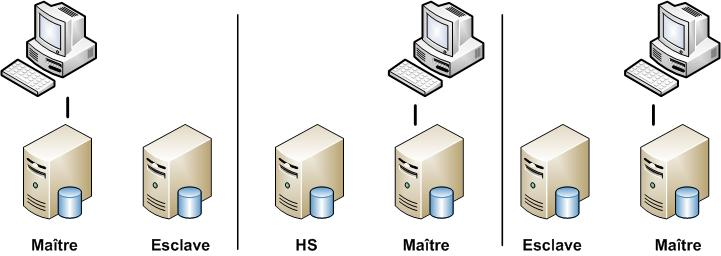
\includegraphics[width=\linewidth]{./Dessin1.jpg}

Un nœud est désigné maître, il gère le service et tout ce qui ce passe sur lui
est répliqué sur le nœud désigné esclave. \\

Si le nœud maître tombe, l’esclave prend le relais. Lorsque le nœud anciennement
maître du cluster sera de nouveau opérationnel, il sera désigné comme esclave. \\ 

\textbf{Terminologie :} chaque machine du cluster est appelé un Node ou un Nœud.

\subsection{Actif/Actif}

\begin{center}
  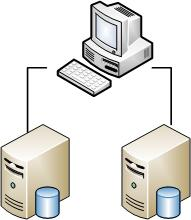
\includegraphics[width=0.3\textwidth]{./Dessin2.jpg}
\end{center}


Dans ce cas il n'y a pas de notion de maître/esclave les nœuds fonctionnent
ensemble et les charges sont réparties sur chaque nœud. \\

Si un nœud tombe toute la charge retombe sur l'autre. \\

\subsection{Journaux de transactions}

Chaque transaction réalisant des modifications sur la structure ou les données
d'une base est tracée dans les journaux de transactions qui contiennent des
informations de bas niveau (comme les blocs modifiés sur un fichier) et non la
requête elle même. \\

Les journaux de transactions sont valables pour toutes les bases de données de
l'instance et sont utilisé en cas de crash du serveur. Lors du redémarrage,
PostgreSQL rejoue les transactions qui n'auraient pas été synchronisées sur les
fichiers de données. \\


\subsection{Warm Standby}

C’est un système de réplication complet qui lorsque que le serveur maître a
terminé de travailler sur un journal de transactions, l’archive sur un second
serveur où il sera récupéré par le serveur PostgreSQL esclave et rejoué dès la
fin de la copie. \\

Deux inconvénients : \\

\begin{itemize}

\item Le délai de prise en compte des modifications dépend de l'activité du serveur
maître (plus ce dernier sera actif, plus il enverra rapidement un journal de
transactions, plus le serveur esclave sera à jour).
\item Le serveur esclave n'est pas disponible, y compris pour des requêtes en
  lecture seule. 
\end{itemize}

Cette technique ne permet de répliquer que l’ensemble des bases de données du
cluster.\\

Cette limitation est liée au fait que les journaux de transactions de PostgreSQL
(aka WALs) tracent toutes les transactions du cluster, quelle que soit la base
de données.\\
 

\subsection{Hot Standby}

C'est une évolution du Warm Standby. Les serveurs esclaves sont désormais
ouverts aux lectures. Ce qui permet aux utilisateurs de PostgreSQL de pouvoir
effectuer des SELECT sur plusieurs répliques de la base PostgreSQL, sans avoir à
utiliser un outil tiers, comme Slony.\\

 Charge à l'application de diriger les requêtes en lecture seule sur l'un ou
 l'autre des esclaves. \\


\subsection{Propriétés ACID}


Les propriétés ACID (atomicité, cohérence, isolation et durabilité) sont un
ensemble de propriétés qui garantissent qu'une transaction est exécutée de façon
fiable.\\

L’atomicité c’est assurance qu'une transaction se fait au complet ou pas du tout
La cohérence c’est assurance que chaque transaction amènera le système d'un état
valide à un autre état valide.\\

L’isolation c’est assurance que l'exécution simultanée de transactions produit
le même état que celui qui serait obtenu par l'exécution en série des
transactions.\\

La durabilité c’est assurance que lorsqu’une transaction a été confirmée, elle
demeure enregistrée même à la suite d'une panne d'électricité, d'un
disfonctionnement de l'ordinateur ou d'un autre problème.


\section{Différents types de réplication}


\subsection{Définition}

La réplication a pour principal but d’avoir un second serveur, sur lequel
travailler en cas de panne du premier. De cette manière l'activité n’est pas
impactée par la perte d'un serveur.\\

Le serveur secondaire peut aussi servir à y déporter une partie du travail afin
d'alléger la charge du serveur principal. Pour cela, plusieurs types de
réplication existent.\\

\subsection{Asynchrone}

\subsubsection{Asymétrique}

\begin{center}

\includegraphics[width=0.75\textwidth]{./Dessin3.jpg}
\end{center}

Un serveur maître est en lecture/écriture alors que le ou les serveurs esclave
ne sont disponibles qu’en lecture. \\

Tout enregistrement fait sur le maître n'est pas immédiatement reporté sur
l'esclave et c’est un processus extérieur au SGBD qui gère la réplication. \\

Si le serveur maître tombe en panne avant de transférer les dernières
transactions au(x) serveur(s) esclave(s), les données de ces transactions y
seront absentes. \\

La réplication interne de PostgreSQL , Slony, Londiste… permettent de mettre en
place ce type de réplication.\\

\subsubsection{Symétrique}

\begin{center}

\includegraphics[width=0.75\textwidth]{./Dessin4.jpg}
\end{center}

Les serveurs sont tous en lecture/écriture. Il faut donc pouvoir gérer les
conflits causés par la mise à jour des mêmes objets sur plusieurs serveurs en
même temps. Cela complexifie de beaucoup le respect de la norme ACID car si une
copie échoue alors que la transaction a déjà été validée, on peut alors arriver
dans une situation où les données sont incohérentes entre les serveurs. \\

Bucardo implémente ce type de système sur deux serveurs uniquement. \\

\subsection{Synchrone}

\subsubsection{Asymétrique}

\begin{center}

\includegraphics[width=0.75\textwidth]{./Dessin5.jpg}
\end{center}

Il n'y a qu'un seul maître mais chaque modification réalisée sur le maître doit
être enregistrée sur l'esclave avant de redonner la main à l'utilisateur. Ce qui
est source de lenteurs car deux systèmes enregistre l'information au lieu d'un
seul  (plus lags réseau possibles) cependant cela permet de ne pas perdre de
donnée en cas d’arrêt du maître. \\

Cela ne résout pas pour autant tous les problèmes car cette solution garantit
seulement que les données est enregistrées sur les esclaves, pas qu’elles soient
visible. Donc en cas de répartition de charge, il est possible qu'une lecture du
maître et de l'esclave ne donnent pas le même résultat. \\

La réplication interne de PostgreSQL propose cette méthode, pgPool-II le propose
également via son mode de réplication. \\

\subsubsection{Symétrique}

\begin{center}

\includegraphics[width=0.75\textwidth]{./Dessin6.jpg}
\end{center}

Ce mode de réplication est le plus complexe et le plus lent. La complexité est
due à la gestion des conflits, inévitable quand il y a plusieurs serveurs
maîtres. La lenteur est due au côté synchrone du système.

À ce jour, Postgres-XC est le projet le plus sérieux de réplication synchrone
symétrique pour PostgreSQL.


\section{La haute disponibilité et le failover}

\subsection{Cluster Haute Disponibilité (fail over)}

Les clusters dits à haute disponibilité ont été créés pour prévenir contre les
failles hardware et software d'une seule machine.

Ainsi, dans ce type de système, si le nœud primaire (ou maître) venait à
rencontrer une défaillance, il sera immédiatement remplacé par le nœud
secondaire (esclave), mis en état de "sommeil" en attendant. Typiquement, ce
second nœud n'est ni plus ni moins qu'une image exacte du nœud primaire et ceci
afin qu'il puisse usurper l'identité du primaire et garder ainsi l'environnement
inchangé pour un utilisateur extérieur. 

\subsection{Cluster à répartition de charge (load balancing)}

Les systèmes à répartition de charge permettent de distribuer l'exécution de
processus systèmes ou réseaux à travers les nœuds du cluster. \\

Le nœud server se voit ainsi attribuer la tâche de réceptionner le processus et
de le répartir sur la machine adéquate. Cette dernière est en fait choisie car
sa charge est faible et donc elle peut traiter le processus entrant de manière
quasi instantanée. Elle peut aussi être choisie en fonction de sa
spécialisation. \\

Ces systèmes requièrent des applications qui examinent la charge courante des
nœuds et déterminent quel nœud pourra résoudre de nouvelles requêtes. Ainsi,
chaque machine se verra attribuer un processus et donc la qualité de service
rendu s'en trouvera meilleure. De plus, il évite les surcharges que peut subir
une seule machine destinée à répondre aux requêtes du réseau. \\


\chapter{Le clustering — deux approches différentes avec le libre}
\section{Bucardo}
\subsection{Identité}

Bucardo est né de la volonté d'une entreprise de l'Utah aux Etats-Unis,
Backcountry, important fournisseur d'équipements de plein air, de pouvoir
synchroniser ses différentes bases de données sous postgresql, dans des délais
les plus brefs possibles, sans pour autant qu'il faille du temps réel. Ses
dirigeants se tournèrent vers une autre entreprise spécialisée, End Point, afin
de trouver une solution à leur projet. \\

La première mise en service véritablement fiable de Bucardo fût réalisée en
2002, des millions de lignes de différentes bases commencèrent à être
répliquées. \\

En 2006, Bucardo fût redéveloppé, afin de s'appuyer sur des fonctionnalités
nouvelles, des techniques plus modernes avec des outils plus récents, comme le
fonctionnement basé sur des démons, des fichiers de log et de configuration plus
flexibles, la gestion de conflits d'écritures sur les tables, ou bien encore
l'ajout de routines pour la gestion d'exception. \\

Les performances s'en trouvèrent nettement améliorées et des mécanismes
d'auto-maintenance furent ajoutés. \\

Bucardo fonctionne chez Backcountry depuis 2006.
En Septembre 2007, le code source de la version 3.0.6 de Bucardo fût couvert par
la même licence que Posgresql, à savoir la licence BSD, autrement dit, Bucardo
devient alors un projet libre. Un site internet fût créé pour l'occasion, dont
l'adresse est www.bucardo.org. Il existe d'assez nombreux contributeurs à ce
projet, mais Greg Sabino Mulane est le principal développeur. \\

Bucardo en est aujourd'hui à sa version 4.5.0 stable, il supporte les moteurs de
postgresql à partir de la version 8, mais il faut savoir qu'une version beta
4.99.8 préfigure ce que sera la version 5.0 à venir. \\

Juste pour information, de profondes modifications auront lieu dans la version
5, et, même si l'esprit Bucardo restera le même, la mise en œuvre pourrait être
assez différente de la version 4. \\



\subsection{Fonctionnalités intégrées et intégrables}

Bucardo est donc un système de réplication de bases de données, ou de clustering
pour les accros des termes anglo-saxons. Son mode fonctionnement est du type
“asynchrone – symétrique”, autrement dit, Bucardo peut aussi bien fonctionner en
mode “master/master” qu'en “master/slave”. Alors que Bucardo peut gérer
plusieurs serveurs en mode esclave, il ne peut gérer plus de deux serveurs en
mode maître. \\

Par ailleurs, contrairement à d'autres systèmes de réplication comme pgPool par
exemple, Bucardo fonctionne en mode asynchrone, car en effet, il s'appuie sur
des composants extérieurs à postgresql pour parvenir à ses fins, de plus,
Bucardo n'utilise nullement les mécanismes des wal files de postgresql par
exemple, il gère lui-même les modifications apportées aux différentes tables des
différentes bases dont il a la surveillance. Dans la terminologie de Bucardo, on
parle de “deltas”, autrement dit, Bucardo consigne les variations entre les
tables de la base, et les images des tables qu'il prend en charge. D'ailleurs,
chaque base de données surveillée par Bucardo possède sa propre base Bucardo,
mais également un schéma supplémentaire Bucardo associé aux propres schémas de
la base en question. \\


En outre, on voit bien que Bucardo intègre tous les ingrédients inhérents à la
répartition de charge ou bien encore aux mécanismes de basculement en cas
d'anomalie, mais ne possède pas toutefois ces fonctionnalités intégrées à son
processus d'installation. Mais peu importe, puisqu'il existe de nombreuses
solutions pour parvenir à la mise en oeuvre de “High Availability”, notamment
dans le monde Linux/Unix, et sans tous les citer, on peut très bien déployer de
la haute disponibilité avec Haproxy par exemple, qui est capable de proposer de
la répartition de charge, d'une part, mais également un mécanisme de basculement
automatique en cas de défaillance du bloc maître principal. Bien sûr, Haproxy
devient notre SPOF — pour Single Point Of Failure —, qu'importe, vous pouvez
sécuriser l'infrastructure très facilement, en doublant Haproxy à l'identique, à
l'adresse IP près, et utiliser de façon simple, soit les mécanismes du DNS, soit
encore de façon un peu moins simple, utiliser un produit comme Heartbeat qui
permet de surveiller le bon fonctionnement d'un composant et de basculer
automatiquement vers son double en cas de défaillance. \\


De plus, certains autres produits comme pgPool proposent du pooling de
connexions en standard, ce qui permet d'améliorer assez nettement les
performances intrinsèques du SGBD, en maintenant des connexions clients
ouvertes, car en effet, les temps d'initialisation de connexions lors de
transaction sont assez coûteuses en temps. Ces dispositifs permettent aussi de
contourner les contraintes liées au nombre d'utilisateurs maximum autorisés. Et
à ce sujet, on peut très bien coupler Bucardo avec un outil comme pgBouncer,
autre produit libre, qui permet justement de prendre en charge le pool de
connexions sur chacun des SGBD entrant dans la configuration de notre cluster
piloté par Bucardo. \\


Par contre, en cas de désynchronisation des bases du cluster, suite à une
anomalie sur l'un des host, il n'existe pas de solutions automatisées de
re-synchronisation, d'ailleurs, à ma connaissance, seul le projet Postgrres-R
possède cette fonctionnalité. Cela ne signifie pas non plus que la
resynchronisation ne soit pas possible, heureusement, mais dans ce cas, il sera
nécessaire de mettre en place des scripts, qui, s'appuyant sur Bucardo, bien
entendu, pourront permettre la synchronisation, en fait, la propriété asynchrone
de Bucardo, indique que ses mécanismes externes au SGBD (levons un peu le coin
du voile, — perl —) peuvent tout à fait être accomplis par les “crontab“ du
système ou des commandes manuelles.


\subsection{Technique}

\subsubsection{Présentation}

Comme on l'a vu précédemment, la réplication est de type
“asynchrone-symétrique“. En réalité, tout le principe de réplication de Bucardo
repose sur la définition et la mise en œuvre de triggers ou déclencheurs. Mais
par où commencer, peut-être par l'installation. Voici donc un résumé de
l'installation de bucardo, une installation détaillée figure en annexe. \\

Comme on l'a laissé sous-entendre précédemment, Bucardo est en fait un processus
démon dont la substantifique moelle est le langage perl, et qui a par ailleurs
besoin des modules suivants : \\

\begin{mVerb}
DBI (at least version 1.51) 
DBD::Pg (2.0) 
Sys::Hostname (1.11) 
Sys::Syslog (0.13) 
boolean (pour Bucardo 5.0) 
DBIx::Safe (1.2.4) 
\end{mVerb}

Évidemment, Bucardo a besoin d'une base de données pour y installer son schéma
principal, et cette base de données ne peut-être que Postgresql en version 8.3
ou ultérieure, qui doit être dotée en outre des langages pl/pgsql et pl/perl-U,
perl-U étant la version non bridée du langage perl pour postgresql, c'est-à-dire
que tout élément de la base, système ou autres est accessible au travers de ce
langage. Pl/pgsql doit être présent également, sans quoi la base ne pourrait
être utilisée qu'en mode “cible” synchronisé de type “fullcopy”. \\

Voici en version express, les grandes étapes d'installation de bucardo dans
notre cluster : \\

\begin{mVerb}
Install DBIx::Safe and booleani
Download and untar the latest Bucardo
perl Makefile.PL && make && sudo make install
bucardo_ctl install
\end{mVerb}

La dernière étape de l'installation consiste donc à peupler notre cluster avec
une nouvelle base de données nommée 'bucardo', et à créer un nouveau
super-utilisateur nommé lui aussi 'bucardo'. A cette étape, vous obtenez la
fenêtre suivante : \\

\begin{mVerb}
This will install the bucardo database into an existing Postgres cluster.
Postgres must have been compiled with Perl support,
and you must connect as a superuser
 
We will create a new superuser named 'bucardo',
and make it the owner of a new database named 'bucardo'
 
Current connection settings:
1. Host:          <none>
2. Port:          5432
3. User:          postgres
4. Database:      postgres
5. PID directory: /var/run/bucardo
\end{mVerb}

Il suffit de renseigner les quelques informations demandées, host, port, user,
etc... et le tour est joué. D'ailleurs, l'utilisateur 'postgres' est nécessaire
car bucardo se connecte à la base avec ce login pour continuer son
installation. En tout cas, il est souhaitable de paramétrer le compte postgres
en mode trust dans le fichier de configuration de postgresql pg\_hba.conf, au
moins durant l'installation de bucardo. Il est important de noter qu'en ce qui
concerne les host passifs ou slave du cluster, nul besoin d'installer bucardo,
en revanche, il faut tout de même y créer un rôle de connexion nommé bucardo. En
cas d'erreur durant cette installation de bucardo, il est conseillé de reprendre
l'installation du début avec bucardo\_ctl install, mais seulement après avoir
complètement nettoyé la base de tout ce qui concerne bucardo, à l'aide de 'drop'
cascadés notamment. \\

Une remarque s'impose également quant à l'architecture de notre cluster, c'est
que la base de contrôle Bucardo peut-être installée sur une machine différente
de celle dont on veut répliquer les données, cela dit, on gagnera en performance
sur des échanges à base de socket que d'échanges sur le réseau ethernet par
exemple, mais il faut tout de même avoir à l'esprit que l'utilisation de Bucardo
sur une configuration n'est pas neutre en termes de ressources mémoire ou disque
ou processeur. A titre d'information, il faut compter à peu près 200 ko de
mémoire vive par synchronisation, et du temps machine pour les processus perl
dédiés à Bucardo. \\

Supposons donc que notre installation Bucardo soit terminée, une commande
importante qu'il est bon de connaître afin d'avoir une vue d'ensemble de tous
les paramètres de Bucardo, la voici donc : \\

\begin{mVerb}
bucardo_ctl show all
audit_pid                 = 0
autosync_ddl              = newcol
bucardo_current_version   = 4.5.0
bucardo_version           = 4.5.0
ctl_checkabortedkids_time = 30
ctl_checkonkids_time      = 10
ctl_createkid_time        = 0.5
ctl_nothingfound_sleep    = 0.2
ctl_pingtime              = 600
default_email_from        = master@postgresql-centos-master.exponentielhippy.fr
default_email_host        = 10.11.12.251
default_email_to          = admin@zimbra.exponentielhippy.fr
email_debug_file          =
endsync_sleep             = 1.0
host_safety_check         =
kid_abort_limit           = 3
kid_abort_sleep           = 1
kid_nodeltarows_sleep     = 0.8
kid_nothingfound_sleep    = 0.3
kid_pingtime              = 60
kid_serial_sleep          = 10
log_conflict_details      = 0
log_conflict_file         = bucardo_conflict.log
log_showline              = 0
log_showpid               = 0
log_showtime              = 3
max_delete_clause         = 200
max_select_clause         = 500
mcp_dbproblem_sleep       = 15
mcp_loop_sleep            = 0.1
mcp_pingtime              = 60
piddir                    = /var/run/bucardo
reason_file               = bucardo.restart.reason.log
stats_script_url          = http://www.bucardo.org/
stopfile                  = fullstopbucardo
syslog_facility           = LOG_LOCAL1
tcp_keepalives_count      = 0
tcp_keepalives_idle       = 0
tcp_keepalives_interval   = 0
warning_file              = bucardo.warning.log
\end{mVerb}

En tout cas, Bucardo permet la mise en œuvre d'architecture de réplication assez
souple, car au final, vous pourriez envisager d'inclure tout le cluster dans une
seule et même machine, ou aussi bien l'éclater sur différentes machines, à
savoir une base sur une machine, son réplicat, pour reprendre un terme propre à
la biologie de l'ADN, sur une autre, et la base principale de contrôle Bucardo
sur une autre encore. \\


En fait, toutes les informations dont a besoin ce démon contrôleur Bucardo sont
comprises dans la base de données principale nommée bucardo, elle contient toute
information utile à la réplication, à savoir la localisation des bases sur le
réseau par exemple, quelles tables sont concernées dans la réplication, quels
types de réplication ont été programmés, et bien d'autres informations encore ;
voici ci-dessous l'exemple d'une base de données test1, créé à l'aide pgbench, et
pour laquelle nous allons bâtir notre cluster : \\

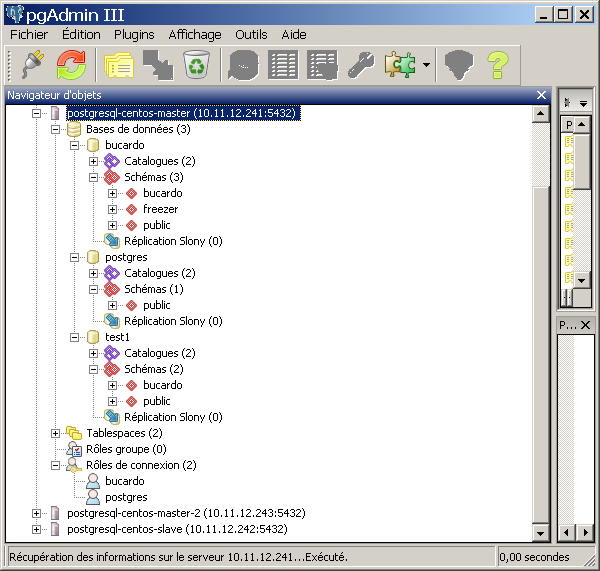
\includegraphics[width=\linewidth]{./pgadmin.png}

Vous pouvez noter la présence d'une base bucardo, mais également des schémas
bucardo pour notre base test1, notez également le schéma freezer de la base
principale bucardo, qui contient l'archivage des actions de réplication qui ont
été menées jour après jour. D'ailleurs, dans ce schéma est créé une table par
jour d'utilisation de la base, il faut donc prévoir une politique de nettoyage
sans quoi la base peut devenir énorme, et apporter son lot de ralentissement à
l'ensemble du SGBD. \\


Sur la vue suivante, vous pouvez constater la présence de tous les composants de
base d'un SGBD dans la base bucardo, des tables, des séquences, des fonctions,
des triggers, etc … mais jugez plutôt, on note la présence de 13 fonctions,
certaines écrites plpgsql, d'autres en pur sql, et aussi quelques unes écrites
en plperl-U, qui s'occupent de tout ce qui se rapporte aux échanges avec le
monde extérieur à la base, comme la gestion des connexions par exemple. C'est
d'ailleurs pourquoi on parle de liaisons asynchrones dans la réplication, car
lorsque Bucardo traite les modifications de la base avec les systèmes
répliqués, les transactions sur les données de la base test1 ont déjà eu
lieu. Ce qui occasionne bien évidemment des délais de propagation et de mise à
disposition de l'information répliquée, de l'ordre de 1 à 5 secondes, mais aussi
des problèmes de synchronisation en cas d'échec de la transaction de réplication
par exemple. Ces délais de réplication peuvent évidemment varier en fonction des
accès réseaux et des configurations matérielles, nos tests ont été effectués sur
des VM guest situées sur la même VM host. \\

On note aussi la présence d'une palanquée de tables contenant les informations
de configuration de nos réplications, et également des tables nécessaires au
fonctionnement de Bucardo, comme par exemple la table 'q' qui contient la liste
des réplications qui ont eu lieu, une ligne par action, avec des infos comme le
nom de la synchronisation, les tables concernées, la nature de la réplication,
la date de début ou de fin, le pid et le ppid des processus engendrés, etc… \\

Enfin, on note la présence de déclencheurs qui, eux aussi, sont soit écrits en
plpgsql, soit en plperl-U et dont les missions  sont aussi diverses que gérer
des logs, ou bien encore valider une réplication ou bien encore vérifier la
configuration de Bucardo. \\

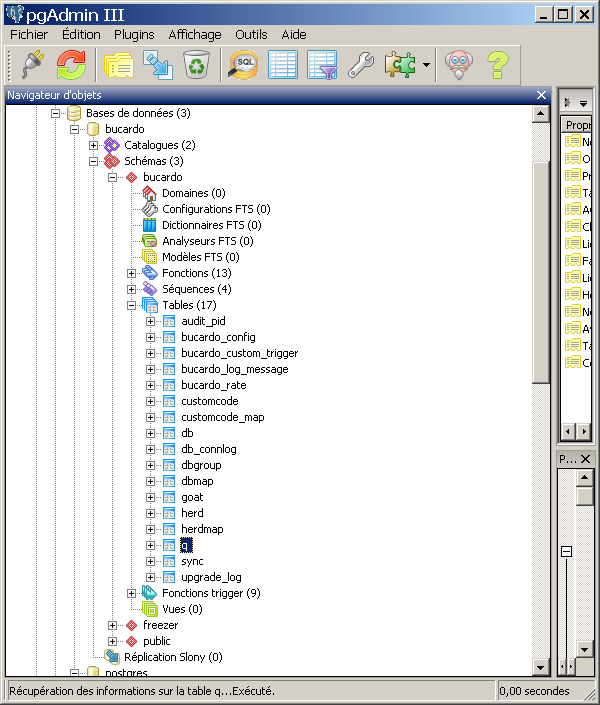
\includegraphics[width=\linewidth]{./pgadmin2.png}

Remarquez bien le nom des tables, nous allons en reparler un peu plus loin. \\

Le décor est planté, alors, que propose Bucardo, c'est ce que nous allons
découvrir. \\

Bucardo est donc un système de réplication de bases de données pour Postgresql,
et en son sein, on découvre trois types de réplication, à savoir un type
'fullcopy', un type 'pushdelta' et un type 'swap'. Faisons les présentations. \\


Le type de réplication 'fullcopy' de Bucardo consiste simplement à recopier le
contenu intégral d'une table, depuis la source vers la cible, après que la table
correspondante sur l'hôte cible ait été vidée de son contenu. D'ailleurs, cette
technique de réplication s'appuie sur la commande Postgresql 'copy'. Dans
Bucardo, c'est en fait le seul mode de réplication dont on dispose lorsque la
table à répliquer ne possède ni clé primaire, ni index unique. De plus,
considérant que la réplication consiste à copier la table dans son intégralité,
il est clairement contre-indiqué d'utiliser cette technique sur des tables
complexes contenant trop de lignes. Autrement dit, si le cas se présente, il
vaut mieux ajuster un index sur ladite table et utiliser une autre technique,
comme celle que nous allons voir immédiatement. \\


Bucardo offre aussi la possibilité de réplication de type 'pushdelta', Cette
synchronisation entraîne la réplication des seules lignes de la ou des tables
qui ont été modifiées, depuis la source, on dit aussi le maître, vers la cible,
que l'on qualifie aussi d'esclave. Pour en revenir à la source, effectivement,
elles peut contenir plusieurs tables, mais également des séquences, et de plus,
en ce qui concerne la cible, il peut s'agir d'un ou plusieurs hôtes esclave,
car, rappelons-le, Bucardo est un système de réplication multi-slave, en plus
d'être multi-maître. Cette granularité dans ce mode de réplication impose comme
contrainte fondamentale que la ou les tables possèdent au moins une clé primaire
ou bien encore un index unique. Ce fait est incontournable, car, sans cela, il
est impossible de créer un 'sync' de type 'pushdelta'. \\

Bien entendu, avant la mise en œuvre de cette réplication, on peut initialiser
l'hôte esclave en peuplant les tables concernées, soit par une méthode classique
de type pg\_dump, soit également, en utilisant Bucardo et le script 'pushdelta'
qui vous avez créé, avec l'option onetimecopy=2, ce qui impliquera une copie
intégrale des tables concernées plutôt que la simple copie des données
modifiées. Cela peut s'avérer très utile aussi au cas où il faudrait
re-synchroniser les tables du cluster. Commençons à nous familiariser avec la
syntaxe Bucardo, et pour cela, voici les commandes de synchronisation
complète : \\

\begin{mVerb}
bucardo_ctl update sync <syncname> onetimecopy=2
bucardo_ctl reload <syncname>
\end{mVerb}

Dès que la commande 'reload' est lancée, l'exécution débute, et le paramètre
'onetimecopy' du sync 'syncname' repasse à 0, car c'est le paramètre par défaut
du 'pushdelta', à savoir, la recopie des modifications uniquement. \\

Encore une précision, les deux commandes ci-dessus sont effectuées dans votre
shell préféré bien entendu, autrement dit, vous avez le contrôle du Bucardo par
l'intermédiaire de votre shell, ce qui peut présenter de réels intérêts ,
notamment si l'on doit effectuer des tâches 'cron' particulières.Vous pourriez
par exemple très bien programmer durant la nuit un traitement de
resynchronisation vers le serveur slave de tous vos script de type 'pushdelta'. \\

Autrement dit, nous transformons ainsi notre 'sync' d'un type 'pushdelta' en un
type 'fullcopy'.\\


Maintenant que nous venons de préciser les deux méthodes de synchronisation
'fullcopy' et 'pushdelta', nous avons bien là les moyens techniques de bâtir une
infrastructure de réplication de nature 'master/multi-slave'. Voyons à présent
la troisième méthode de réplication que propose Bucardo, à savoir le type
'swap'.\\


Bucardo a ceci d'intéressant qu'il est capable de gérer des réplications du type
'swap', c'est-à-dire de la réplication de tables entre deux SGBD de façon
bi-directionnelle, en réalité, nous avons là, à notre disposition, un moyen de
proposer une architecture de type 'master/master', mais entendons nous bien,
cela n'est possible que sur un ensemble de deux maîtres et seulement deux. De la
même façon que la réplication de type 'pushdelta', la réplication de type 'swao'
ne peut se faire qu'entre des tables qui possèdent au moins une clé primaire ou
bien encore un index unique. Il est vrai que dans le cas où notre base
contiendrait des tables sans index unique, il faudrait en passer par de la
gestion en mode 'fullcopy', avec les contraintes que ça implique, comme on l'a
expliqué plus haut. Et bien entendu, qui dit réplication de type actif/actif,
dit aussi conflits d'écritures. Heureusement, dans Bucardo, on a à notre
disposition plusieurs manières de gérer les conflits ; il faut tout d'abord
définir, parmi nos deux 'hosts', lequel est la source et lequel est la cible
(target), il n'y a pas de règles particulières, ce choix est laissé à
l'initiative de l'administrateur, il peut par exemple décider que la source est
le serveur le plus performant, pourquoi pas, puis vient ensuite la définition de
notre réplication de type 'swap', pour laquelle on décide par exemple qu'en cas
de conflit, c'est la source qui prévaut, mais on peut aussi paramétrer cet
ensemble de réplication en indiquant que c'est la cible qui gagne. Bucardo nous
propose d'ailleurs en standard d'autres choix possibles, mais voici la liste
complète : \\

\begin{mVerb}
source – les lignes de la source l'emportent et la copie à lieu de la source vers la cible
target – les lignes de la cible l'emportent.
skip – on néglige la réplication en cas de conflit (peu recommandé)
random – choix aléatoire avec la même probabilité que le pile ou face.
latest – la ligne la plus récemment modifiée l'emporte.
abort – la réplication s'interrompt en cas de conflit.
\end{mVerb}

Mais mieux encore, Bucardo est si ouvert qu'il permet également de définir ses
propres directives de gestion des conflits, au cas où notre modèle conceptuel de
données exigerait des traitements non prévus en standard. \\


Nos trois mécanismes de réplication viennent d'être présentés, et à présent,
on pourrait passer aux travaux pratiques, en présentant de façon succincte le
déroulement de la définition d'une réplication, en commençant par une
réplication de type master/slave, puis ensuite en poursuivant avec une
réplication de type master/master. \\


Bucardo est un outil vraiment très flexible, puisque comme on le disait
précédemment, il peut être installé n'importe où, sur une machine dédiée ou pas,
nous avons choisi trois machines virtuelles avec Postgresql 8.4 sous une
distribution Centos 6, chacune abritant la même base de données, à savoir celle
qui est installée avec le produit pgbench. Pour mémoire, pgbench est l'outil mis
à disposition des utilisateurs de Postgresql-contrib afin d'effectuer des tests
de robustesse des SGBD. Il s'appuie sur les définitions du TPC-B (Transaction
Processing Performance Concil). \\

Pour commencer, il faut peupler nos bases Postgresql 8.4 sur chacune des VM, qui
se situent aux adresses réseaux 10.11.12.241 pour le premier maître dit la
'source', 10.11.12.242 pour le serveur esclave, et enfin 10.11.12.243 pour le
deuxième maître qui aura un rôle de 'cible'. \\

Pour cela, rien de plus simple, il suffit de lancer les commandes suivantes, en
créant d'abord nos bases sur chacun des host, en sous-entendant que x vaut 1, 2
ou 3, vous vous en doutez : \\

\begin{mVerb}
createdb -h 10.11.12.24x -p 5432 -U postgres test1
\end{mVerb}

puis en peuplant la base de données avec pgbench : \\

\begin{mVerb}
pgbench -i -h 10.11.12.24x -p 5432 -U postgres test1
\end{mVerb}

où test1 est le nom de notre base de données, vous l'aurez sans doute déjà
remarqué dans les figures ci-dessus. \\

Les composants de notre infrastructure sont donc prêts. Voici d'ailleurs le
contenu de nos bases, avec la commande suivante :  \\

\begin{mVerb}
psql -h 10.11.12.24x -p 5432 -U postgres -d test1 -c "\dt+" 

                           Liste des relations
 Schéma |       Nom        | Type  | Propriétaire | Taille  | Description
--------+------------------+-------+--------------+---------+-------------
 public | pgbench_accounts | table | postgres     | 27 MB   |
 public | pgbench_branches | table | postgres     | 24 kB   |
 public | pgbench_history  | table | postgres     | 1304 kB |
 public | pgbench_tellers  | table | postgres     | 152 kB  |
(4 lignes)
\end{mVerb}

Parmi ces tables, seule la table pgbench\_history ne possède pas d'index unique,
elle est le reflet des transations effectuées sur les autres tables, c'est un
historique en fait. Elle peut toutefois contenir un grand nombre de lignes. \\

La table pgbench\_accounts contient 100000 lignes, la table pgbench\_tellers en
contient 10 et enfin, la table pgbench\_branches contient une ligne. \\

Parmi ces tables, seule la table pgbench\_history ne possède pas d'index unique,
elle est le reflet des transactions effectuées sur les autres tables, c'est un
historique en fait. Elle peut toutefois contenir un grand nombre de lignes. \\

La table pgbench\_accounts contient 100000 lignes, la table pgbench\_tellers en
contient 10 et enfin, la table pgbench\_branches contient une ligne. \\

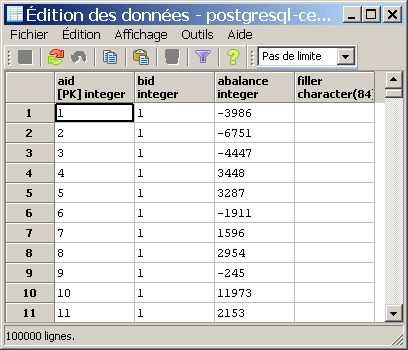
\includegraphics[width=0.5\textwidth]{./pgadmin3.png}
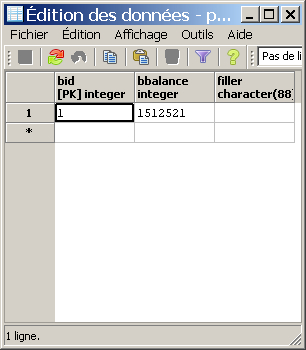
\includegraphics[width=0.5\textwidth]{./pgadmin4.png}
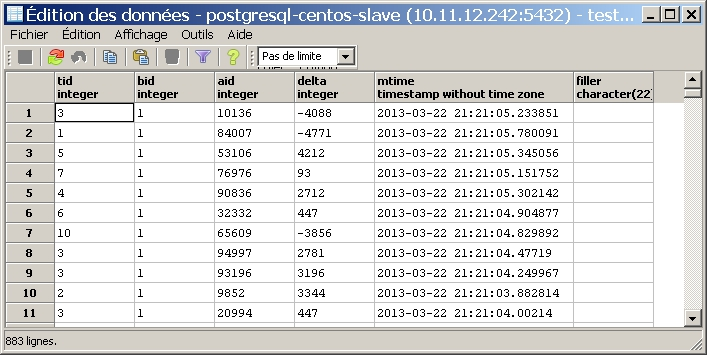
\includegraphics[width=\linewidth]{./pgadmin5.png}
\begin{center}
  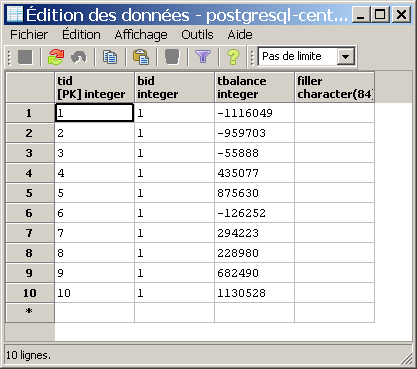
\includegraphics[width=0.5\textwidth]{./pgadmin6.png}
\end{center}


Toutes les briques du puzzle de la réplication sont définies, nous pouvons
désormais présenter la réalisation des différents mode réplication.


\subsection{Réplication cluster actif/passif}

Nous supposons donc que nos trois VM sont démarrées, que nos trois bases
Postgresql ont été lancées par une commande du type :

\begin{mVerb}
/usr/bin/pg_ctl -D /var/lib/pgsql/data/ -l logfile start
\end{mVerb}

Plaçons-nous sur le host master à l'adresse 10,11,12,241, et commençons les
paramètrages de Bucardo en lui indiquant tout d'abord quels sont les bases de
données concernées par cette réplication maître/esclave, et où elles se trouvent
sur le réseau : \\

\begin{mVerb}
bucardo_ctl add database test1 name=test1_master port=5432 host=10.11.12.241
bucardo_ctl add database test1 name=test1_slave port=5432 host=10.11.12.242
\end{mVerb}

Remarquez à nouveau que notre ensemble de commande commence par 'bucardo\_ctl',
et d'ailleurs, il en sera ainsi jusqu'au bout, car c'est le point d'entrée des
instructions avec Bucardo. Vous trouverez d'ailleurs en annexe un listing des
principales commandes bucardo. Si je résume en français la commande ci-dessus,
je demande à bucardo d'ajouter la base test1 située sur le host 10.11.12.24x,
accessible par le port 5432 et cette base de données est baptisée test1\_master ou
test1\_slave, le nom étant choisi comme bon vous semble. En outre, on ne le
précise pas, mais l'utilisateur par défaut est 'bucardo' et dans notre cas, il
n'aura pas de mot de passe, mais bien entendu, en production, ce n'est pas
recommandé. Ainsi, de façon simple, nous venons de définir notre source et notre
cible, mais ce n'est pas tout. Poursuivons à présent en déterminant ce que nous
allons répliquer. \\

Dans notre cas, nous voulons une synchronisation de toute la base test1 sur le
slave, c'est-à-dire une réplication de toutes les tables, mais souvenez-vous que
nous avons une table qui ne possède pas de clé primaire, à savoir la table
pgbench\_history, c'est pourquoi nous allons devoir procéder en deux étapes de
synchronisation, et pour cela, nous allons devoir créer deux sous-ensembles de
notre base test1, l'un avec les tables à index unique, l'autre pour la table
sans index unique. Dans la terminologie de Bucardo,  on appelle ces ensembles
des 'herd', ce que l'on peut traduire par des hardes en français. Vous finirez
par comprendre pourquoi ce terme, si vous êtes un peu familier avec la langue de
Cervantes. \\

Nous allons donc déterminer les hardes alpha et beta, alpha contiendra toutes
les tables à index unique, tandis que beta sera celle de la table sans index
unique, à savoir pgbench\_history, voici comment on procède : \\

\begin{mVerb}
bucardo_ctl add all tables db=test1_master -T pgbench_history --herd=alpha
bucardo_ctl add all tables db=test1_master -t pgbench_history --herd=beta
\end{mVerb}


L'option -T de la première ligne indique que nous prenons toutes les tables de
la base test1, dont la source est test1\_master définie ci-avant, à l'exception
de la table pgbench\_history, et l'option -t indique que nous prenons le
complémentaire de l'ensemble alpha parmi toutes les tables de la source, à
savoir, pgbench\_history.

Voilà, nous venons de définir très simplement, encore une fois, nos deux
sous-ensembles, nos deux hardes. Nous savons à présent ce que nous devons
synchroniser, il ne nous reste plus qu'à définir la nature de nos deux
réplications correspondant à nos deux 'herd', et vous l'aurez deviné, il
convient d'ajuster deux synchronisations, l'une du type 'pushdelta' ayant comme
source notre 'herd' alpha, l'autre du type 'fullcopy' ayant comme source notre
'herd' beta. Et bien, voilà comment on réalise ses deux opérations : \\

\begin{mVerb}
bucardo_ctl add sync benchdeltaalpha source=alpha targetdb=test1_slave 	type=pushdelta
bucardo_ctl add sync benchcopybeta source=beta targetdb=test1_slave 	type=fullcopy
\end{mVerb}


Sur la première ligne, nous ajoutons une synchronisation de nom benchdeltaalpha,
dont la source est bien notre harde alpha, dont la cible test1\_slave est
évidemment notre serveur esclave test1 à l'adresse 10.11.12.242, et de plus,
cette 'sync' pour reprendre la terminologie bucardo est de type 'pushdelta',
quant à la deuxième ligne, elle précise qu'il s'agit d'une synchronisation de
type 'fullcopy' de notre 'herd' beta vers la cible de nom test1\_slave. \\

Vous l'aurez noté, la simplicité avec laquelle nous venons de créer un cluster
actif/passif est assez déconcertante. Et pour ne pas se priver de notre plaisir,
on peut vérifier par quelques commandes simples le résultat de nos tâches, et
ainsi voir si tout est bien en place pour mettre notre cluster en fonction,
voici donc quelques commandes utiles Bucardo :

\begin{mVerb}
bucardo_ctl list db
Database: test1_master   Status: active  Conn: psql -p 5432 -U bucardo -d test1 -h 10.11.12.241
Database: test1_slave    Status: active  Conn: psql -p 5432 -U bucardo -d test1 -h 10.11.12.242
\end{mVerb}

\begin{mVerb}
bucardo_ctl list tables
Table: public.pgbench_accounts  DB: test1_master  PK: aid (int4)
Table: public.pgbench_branches  DB: test1_master  PK: bid (int4)
Table: public.pgbench_history   DB: test1_master  PK: none
Table: public.pgbench_tellers   DB: test1_master  PK: tid (in
\end{mVerb}

\begin{mVerb}
bucardo_ctl list herd
Herd: alpha  DB: test1_master  Members: public.pgbench_branches,
public.pgbench_tellers, public.pgbench_accounts

  Used in syncs: benchdeltaalpha
Herd: beta   DB: test1_master  Members: public.pgbench_history
  Used in syncs: benchcopybeta
\end{mVerb}

\begin{mVerb}
bucardo_ctl list sync
Sync: benchcopybeta    (fullcopy )  beta  =>  test1_history  (Active)
Sync: benchdeltaalpha  (pushdelta)  alpha =>  test1_slave    (Active)
\end{mVerb}

Tout semble parfaitement en ordre, il ne nous reste plus qu'à lancer le
clustering master/slave, et voici comment : \\

\begin{mVerb}
bucardo_ctl start
\end{mVerb}

Après quelques messages d'activation, le prompt réapparaît et notre instance
Bucardo est activée, d'ailleurs, vous pouvez vérifier cela en lisant le fichier
log.bucardo et en vérifiant les processus lancés de cette façon : \\

\begin{mVerb}
ps ax | grep -i bucardo

11801 ?        S      3:36 Bucardo Master Control Program v4.5.0. Active syncs:
benchcopybeta,benchdeltaalpha
11802 ?        Ss     0:02 postgres: bucardo bucardo [local] idle
11804 ?        Ss     0:05 postgres: bucardo test1 10.11.12.241(55424) idle
11805 ?        S      1:34 Bucardo Controller. Sync "benchcopybeta" (fullcopy) for source "beta"
11806 ?        S      1:33 Bucardo Controller. Sync "benchdeltaalpha"
(pushdelta) for source "alpha"
11807 ?        Ss     0:04 postgres: bucardo bucardo [local] idle
11808 ?        Ss     0:03 postgres: bucardo bucardo [local] idle
11809 ?        S      1:00 Bucardo Kid. Sync "benchcopybeta": (fullcopy)
"test1_master" -> "test1_master2"
11810 ?        S      0:58 Bucardo Kid. Sync "benchdeltaalpha": (pushdelta)
"test1_master" -> "test1_slave"
11811 ?        Ss     0:01 postgres: bucardo bucardo [local] idle
11812 ?        Ss     0:01 postgres: bucardo bucardo [local] idle
11813 ?        Ss     1:00 postgres: bucardo test1 10.11.12.241(55427) idle
11814 ?        Ss     0:01 postgres: bucardo test1 10.11.12.241(55428) idle
11815 ?        S      1:00 Bucardo Kid. Sync "benchcopybeta": (fullcopy)
"test1_master" -> "test1_slave"
11816 ?        Ss     0:01 postgres: bucardo bucardo [local] idle
11817 ?        Ss     0:01 postgres: bucardo test1 10.11.12.241(55431) idle
\end{mVerb}

Vous constatez que différents processus ont été lancés par Bucardo, dont le
contrôleur principal et les processus de synchronisation. \\

Et c'est à cet instant qu'entre en action, l'outil pgbench pour exercer quels
tirs de requêtes sur notre serveur maître, afin de voir si la réplication se
passe bien. Avant cela, il faut rappeler que notre moteur Postgresql est
paramétré de tel façon qu'il n'accepte pas plus de 100 connexions simultanées,
c'est d'ailleurs le paramètre par défaut dans posgresql.conf. \\

Voici le type de tir avec pgbench que nous effectuerons tout au long de nos
essais :

\begin{mVerb}
./pgbench -h 10.11.12.241 -p 5432 -U postgres -c 20 -C -T 10 test1
starting vacuum...end.
transaction type: TPC-B (sort of)
scaling factor: 1
query mode: simple
number of clients: 20
number of threads: 1
duration: 10 s
number of transactions actually processed: 687
tps = 67.836201 (including connections establishing)
tps = 230.233437 (excluding connections establishing)
\end{mVerb}

Quelques explications sur ce tir, notamment en ce qui concerne les paramètres de
pgbench, nous avons -c 20 pour indiquer le nombre de clients simultanés qui
procède aux tirs, l'option -C pour préciser à pgbench de déclencher une
reconnexion après chaque transaction, ce qui rapproche de l'usage d'un serveur
par un grand nombre de clients différents, puis vient l'option -T pour indiquer
la durée des tirs. D'ailleurs, à propos de l'option -C, elle se repère très bien
lorsque l'on observe le nombre de transactions par seconde, autrement dit, les
temps de connexions/déconnexions sont très pénalisants pour les performances
pures d'accès aux données. A ce titre, c'est la raison pour laquelle certains
outils comme pgPool par exemple, peuvent prendre en charge le pooling de
connexions, afin de rendre persistantes les connexions pour un même client, ce
qui lui évite les déconnexions intempestives, et améliore très nettement le
nombre de tps. Voyons à présent l'état de deux des tables essentielles de notre
master et de notre slave respectivement :

\begin{mVerb}
psql -h 10.11.12.241 -p 5432 -U postgres -d test1 -c "select * from
pgbench_tellers order by tid asc;"

 tid | bid | tbalance | filler
-----+-----+----------+--------
   1 |   1 | -1091845 |
   2 |   1 |  -993331 |
   3 |   1 |   -42076 |
   4 |   1 |   438138 |
   5 |   1 |   906281 |
   6 |   1 |  -198650 |
   7 |   1 |   220693 |
   8 |   1 |   231572 |
   9 |   1 |   721298 |
  10 |   1 |  1113296 |
(10 rows)
\end{mVerb}

\begin{mVerb}
psql -h 10.11.12.242 -p 5432 -U postgres -d test1 -c "select * from pgbench_tellers order by tid asc;"

 tid | bid | tbalance | filler
-----+-----+----------+--------
   1 |   1 | -1091845 |
   2 |   1 |  -993331 |
   3 |   1 |   -42076 |
   4 |   1 |   438138 |
   5 |   1 |   906281 |
   6 |   1 |  -198650 |
   7 |   1 |   220693 |
   8 |   1 |   231572 |
   9 |   1 |   721298 |
  10 |   1 |  1113296 |
(10 rows)
\end{mVerb}

Vérifions aussi le nombre de lignes de la table pgbench\_history qui indique le
nombre de transactions effectuées sur la base : \\

\begin{mVerb}
psql -h 10.11.12.241 -p 5432 -U postgres -d test1 -c "select count(*) from pgbench_history"

 count
-------
   687
(1 row)
\end{mVerb}


\begin{mVerb}
psql -h 10.11.12.242 -p 5432 -U postgres -d test1 -c "select count(*) from pgbench_history"

 count
-------
   687
(1 row)
\end{mVerb}

687 transactions sur les deux tables history et les mêmes valeurs dans la table
tellers. C'est exactement ce que nous cherchions à faire, à noter toutefois que
la réplication master/slave est asynchrone, est que le délai de réplication est
de l'ordre de la seconde sur ce genre de configuration, ce qui est déjà assez
satisfaisant, nous sommes pas forcément dans les meilleurs conditions
matérielles.\\

Et j'en profite également pour présenter de façon un peu plus détaillée la
nature des opérations effectuées par pgbench lors d'une transaction, en voici la
teneur sql :\\

\begin{mVerb}
\set nbranches :scale
\set ntellers 10 * :scale
\set naccounts 100000 * :scale
\setrandom aid 1 :naccounts
\setrandom bid 1 :nbranches
\setrandom tid 1 :ntellers
\setrandom delta -5000 5000

1. BEGIN;
2. UPDATE pgbench_accounts SET abalance = abalance + :delta WHERE aid = :aid;
3. SELECT abalance FROM pgbench_accounts WHERE aid = :aid;
4. UPDATE pgbench_tellers SET tbalance = tbalance + :delta WHERE tid = :tid;
5. UPDATE pgbench_branches SET bbalance = bbalance + :delta WHERE bid = :bid;
6. INSERT INTO pgbench_history (tid, bid, aid, delta, mtime) VALUES (:tid, :bid,
:aid, :delta, CURRENT_TIMESTAMP);
7. END;
\end{mVerb}

D'ailleurs, si l'on précise l'option -S dans la commande pgbench, seule la
requête 3 est effectuée, par contre, avec l'option -N, les requêtes 4 et 5 ne
sont pas générées. Ces deux dernières options allègent évidemment le processus.\\


On peut aussi faire une autre petite vérification toute simple comme la suivante
par exemple :\\

\begin{mVerb}
root@debian:~# psql -h 10.11.12.241 -p 5432 -U postgres -d test1 -c "update
pgbench_tellers set filler='modification' where tid=1;"

UPDATE 1

psql -h 10.11.12.242 -p 5432 -U postgres -d test1 -A -c 'select * from
pgbench_tellers where tid=1;'

tid|bid|tbalance|filler
1|1|-1108556|modification
(1 row)
\end{mVerb}

Notre modification a bien été prise en compte, et c'est tant mieux, mais passons
à notre deuxième mode de réplication à présent.\\


\subsection{Réplication cluster actif /actif}

Comme nous l'indiquions un peu plus tôt, nous allons entreprendre une
réplication de type 'swap' au sens de Bucardo, c'est-à-dire une réplication de
type asynchrone-symétrique, autrement dit, on met en place un cluster
maître/maître.\\

Puisque nous sommes prévoyants, notre deuxième machine maître aussi nommé
master-2 est prête et possède l'adresse IP 10.11.12.243. Bien évidemment,
Bucardo y est déjà installé et comme prétexte à l'utilisation de quelques
commandes utiles de Bucardo, nous allons vérifier que rien n'a encore été fait
avec Bucardo, et voici donc ces commandes :\\



\begin{mVerb}
bucardo_ctl list
Usage: list <type> [options]
Shows information about items in the internal Bucardo database.
The type is one of: code, db, dbgroup, table, sequence, herd, sync, customcode
For more information, run: \$progname help list <type>

bucardo_ctl list code
There are no entries in the 'db' table.
bucardo_ctl list db
There are no entries in the 'db' table.
bucardo_ctl list dbgroup
There are no entries in the 'dbgroup' table.
bucardo_ctl list table
There are no entries in the 'goat' table.
bucardo_ctl list sequence
There are no entries in the 'goat' table.
bucardo_ctl list herd
There are no entries in the 'herd' table.
bucardo_ctl list sync
There are no entries in the 'sync' table.
bucardo_ctl list customcode
There are no entries in the 'db' table.
\end{mVerb}

Comme vous le voyez, on peut lister un grand nombre de composants de Bucardo,
d'ailleurs, avez-vous remarqué dans quelle table de Bucardo sont stockées les
tables et les séquences à répliquer, dans une table nommé 'goat', dont la
traduction en français signifie chèvre, ah bon ? Des hardes ? Des chèvres ?\\


Vous le voyez, tous les composants sont bien vides, il ne nous reste plus qu'à
paramétrer notre cluster. On va choisir comme base source la base située sur
notre master-2 à l'adresse 10.11.12.243, celle sur laquelle nous paramétrons
notre réplication de type 'swap', et comme cible le host master à l'adresse
10.11.12.241, notre maître du cluster précédent. Déterminons à présent ce que
nous allons dupliquer, à l'aide des deux commandes suivantes  et avant cela, la
localisation de nos db : \\

\begin{mVerb}
bucardo_ctl add database test1 name=test1_master2 host=10.11.12.243 port=5432
bucardo_ctl add database test1 name=test1_master host=10.11.12.241 port=5432
\end{mVerb}

\begin{mVerb}
bucardo_ctl add all table -T pgbench_history db=test1_master2
	standard_conflict=target herd=gamma
bucardo_ctl add all tables db=test1_master2 -t pgbench_history herd=eta
\end{mVerb}

Nous venons de déterminer ce que nous allions intégrer à nos réplications, aussi
bien pour le mode 'swap' dans le 'herd' gamma que le mode 'fullcopy' dans le
'herd' eta, Mais considérant que la base master est notre base prioritaire au
niveau des conflits, nous choisissons donc de répliquer également en 'fullcopy'
la table pgbench\_history de master vers master-2. A ce titre, il convient
d'effectuer une modification sur notre master afin d'ajouter dans la source beta
une réplication vers test1\_master2, je le rappelle, notre but étant d'avoir une
véritable réplication de nos deux hosts master et master-2.\\

Il va de soi que la gestion ici de notre table pgbench\_history n'est pas
forcément très cohérente, mais le but est avant tout de maintenir deux bases
parfaitement répliquées. Cela montre toutefois que la mise en cluster
actif/actif doit être envisagée au moment de la création du mcd, sans quoi, on
peut se retrouver avec ce genre d'incohérence à gérer.\\

Voici donc nos deux 'sync' parfaitement définis, la preuve : \\


\begin{mVerb}
bucardo_ctl list sync
Sync: benchcopyeta    (fullcopy)  eta   =>  test1_master  (Active)
Sync: benchswapgamma  (swap    )  gamma <=> test1_master  (Active)
\end{mVerb}

Il ne nous reste plus qu'à lancer notre infratructure de réplication et à lancer
une réplication manuellement pour commencer la synchronisation avant la mise en
production : \\

\begin{mVerb}
bucardo_ctl start
bucardo_ctl kick benchcopyeta 0
bucardo_ctl kick benchswapgamma 0
\end{mVerb}


Le paramètre 0 à la fin de la commande kick <syncname> nous affiche le temps de
réplication, et s'il s'agit d'un entier supérieur à 0 strictement, il devient
le nombre de secondes à attendre avant de lancer la réplication, on ne sait
jamais, ça peut servir. \\

À présent, nous allons réaliser deux tirs croisés avec pgbench, d'abord sur le
master et vérifier les master-2, puis ensuite l'inverse, tirer sur le master-2
et comparer les deux hosts. Voici le résultat : \\

\begin{mVerb}
./pgbench -h 10.11.12.241 -p 5432 -U postgres -c 80 -C -T 10 test1

transaction type: TPC-B (sort of)
scaling factor: 1
query mode: simple
number of clients: 80
number of threads: 1
duration: 10 s
number of transactions actually processed: 733
tps = 69.471430 (including connections establishing)
tps = 208.838335 (excluding connections establishing)
\end{mVerb}


\begin{mVerb}
psql -h 10.11.12.241 -p 5432 -U postgres -d test1 -c 'select count(*) from pgbench_history;'
 count 
-------
   733
(1 row)
\end{mVerb}

\begin{mVerb}
psql -h 10.11.12.243 -p 5432 -U postgres -d test1 -c 'select count(*) from pgbench_history;'
 count 
-------
   733
(1 row)
\end{mVerb}

\begin{mVerb}
psql -h 10.11.12.241 -p 5432 -U postgres -d test1 -c 'select * from
pgbench_tellers order by tid;'

 tid | bid | tbalance | filler 
-+----------------------------
   1 |   1 |  -842896 | 
   2 |   1 |  -966596 | 
   3 |   1 |    50287 | 
   4 |   1 |   330902 | 
   5 |   1 |  1023423 | 
   6 |   1 |  -185580 | 
   7 |   1 |    77489 | 
   8 |   1 |   406761 | 
   9 |   1 |   572894 | 
  10 |   1 |  1191867 | 
(10 rows)
\end{mVerb}

\begin{mVerb}
psql -h 10.11.12.243 -p 5432 -U postgres -d test1 -c 'select * from
pgbench_tellers order by tid;'

 tid | bid | tbalance | filler 
-+-----------------------------
   1 |   1 |  -842896 | 
   2 |   1 |  -966596 | 
   3 |   1 |    50287 | 
   4 |   1 |   330902 | 
   5 |   1 |  1023423 | 
   6 |   1 |  -185580 | 
   7 |   1 |    77489 | 
   8 |   1 |   406761 | 
   9 |   1 |   572894 | 
  10 |   1 |  1191867 | 
(10 rows)
\end{mVerb}

\begin{mVerb}
./pgbench -h 10.11.12.243 -p 5432 -U postgres -c 80 -C -T 10 test1

transaction type: TPC-B (sort of)
scaling factor: 1
query mode: simple
number of clients: 80
number of threads: 1
duration: 10 s
number of transactions actually processed: 899
tps = 85.849820 (including connections establishing)
tps = 245.342651 (excluding connections establishing)

psql -h 10.11.12.241 -p 5432 -U postgres -d test1 -c 'select count(*) from pgbench_history;'
 count 
-------
   899
(1 row)
\end{mVerb}

\begin{mVerb}
psql -h 10.11.12.243 -p 5432 -U postgres -d test1 -c 'select count(*) from pgbench_history;'
 count 
-------
   899
(1 row)

01:24:18-238191045
psql -h 10.11.12.241 -p 5432 -U postgres -d test1 -c 'select * from
pgbench_tellers order by tid;'

 tid | bid | tbalance | filler 
-+-----------------------------
   1 |   1 |  -876952 | 
   2 |   1 | -1001509 | 
   3 |   1 |    54695 | 
   4 |   1 |   344456 | 
   5 |   1 |  1024900 | 
   6 |   1 |  -167785 | 
   7 |   1 |    58387 | 
   8 |   1 |   424655 | 
   9 |   1 |   550530 | 
  10 |   1 |  1143991 | 
(10 rows)
\end{mVerb}

\begin{mVerb}
psql -h 10.11.12.243 -p 5432 -U postgres -d test1 -c 'select * from
pgbench_tellers order by tid;'

 tid | bid | tbalance | filler
   1 |   1 |  -876952 |         
   2 |   1 | -1001509 | 
   3 |   1 |    54695 | 
   4 |   1 |   344456 | 
   5 |   1 |  1024900 | 
   6 |   1 |  -167785 | 
   7 |   1 |    58387 | 
   8 |   1 |   424655 | 
   9 |   1 |   550530 | 
  10 |   1 |  1143991 | 
(10 rows)
\end{mVerb}


Au vu des résultats ci-dessus, nous constatons avec émerveillement que notre
réplication maître/maître a bien foncionné, que l'on tire sur le master ou le
master-2.\\


Bien que nous venons d'effectuer des tirs d'abord sur master en 10.11.12.241
puis sur master-2 en 10.11.12.243, vérifions tout de même ce que nous présente
notre slave en 10.11.12.242 :\\


psql -h 10.11.12.242 -p 5432 -U postgres -d test1  -c 'select * from
pgbench\_tellers order by tid;' \\


\begin{mVerb}
 tid | bid | tbalance | filler
-+-----------------------------
   1 |   1 |  -842896 |
   2 |   1 |  -966596 |
   3 |   1 |    50287 |
   4 |   1 |   330902 |
   5 |   1 |  1023423 |
   6 |   1 |  -185580 |
   7 |   1 |    77489 |
   8 |   1 |   406761 |
   9 |   1 |   572894 |
  10 |   1 |  1191867 |
(10 rows)
\end{mVerb}         

\begin{mVerb}
psql -h 10.11.12.242 -p 5432 -U postgres -d test1  -c 'select count(*) from pgbench_history'

 count
-------
   733
(1 row)
\end{mVerb}

Et bien, si vous comparez ces résultats avec le tir sur le master réalisé
précédemment, vous constaterez que la réplication master/slave est toujours
opérationnelle même avec le cluster actif/actif. \\

Tout cela tombe bien finalement, car nous avons réalisé deux types de cluster,
qui fonctionne simultanément, il est peut être temps d'envisager des fonctions
de haute disponibilité, du genre répartition de charge et basculement en cas
d'anomalie. \\

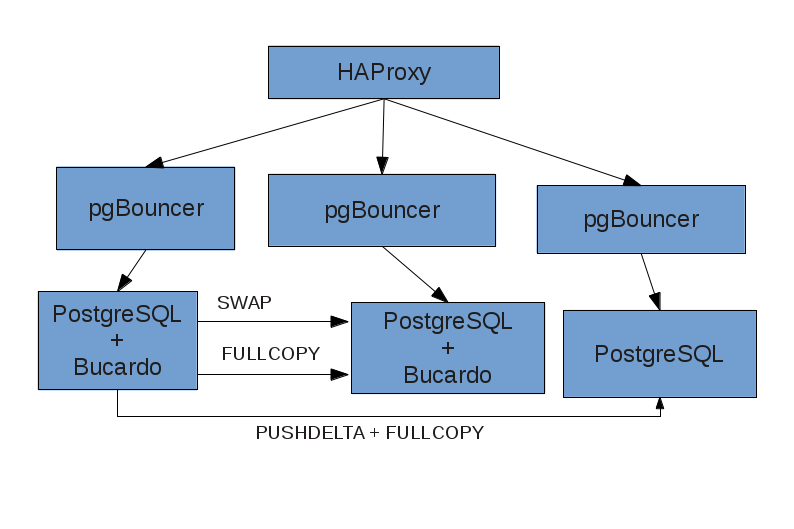
\includegraphics[width=\linewidth]{./arch2.png}

\subsection{En route vers la HA}

Là encore, le monde du libre peut nous proposer des produits très
complémentaires avec notre réplication Bucardo, j'ai nommé haproxy, qui peut
nous permettre de mettre en place de la haute disponibilité en répartissant la
charge sur notre cluster actif/actif, et du basculement ou 'failover' in english
in the text entre nos actifs et notre passif en l'occurence. \\

Et en effet, la mise ne service d'une machine dédiée, sous debian, avec haproxy
nous permet de concevoir notre projet de HA. Voici d'ailleurs quelques
paramètres importants de notre fichier de configuration de notre machine haproxy
à l'adresse 10.11.12.249 : \\


\begin{mVerb}
global
	log 127.0.0.1   local0
	log 127.0.0.1   local1 notice
	maxconn 400
	user haproxy
	group haproxy
	daemon

listen DB_frontend
	bind		10.11.12.249:5432
	mode		tcp
	log		global
	clitimeout	3000 # 9000 sur le port 5432
	balance		roundrobin # le poids varie automatiquement en fonction de la charge
	contimeout	9000 # 9000 sur le port 5432
	srvtimeout	9000 # 9000 sur le port 5432

	# on passe par posgresql directement sur le port 5432
	server         DB_master 10.11.12.241:5432 check inter 1000 weight 10
	server         DB_master-2 10.11.12.243:5432 check inter 1000 weight 10
	server		DB_Slave 10.11.12.242:5432 check inter 1000 weight 10 backup
\end{mVerb}


On retrouve nos trois hosts, et vous noterez les deux masters, qui sont
exploités en backend pour la répartition de charge avec la méthode round robin
avec variation de poids en fonction de la charge de la machine, ceci réalisé
automatiquement par haproxy, et notre host slave en mode backup, ce qui indique
à haproxy qu'en cas d'indisponibilité des deux masters, c'est lui qui prendra le
relais. Ces machines de secours en mode backup pourraient être plus nombreuses
évidemment, et pourraient être exploitées toutes ensembles le cas échéant.\\

D'ailleurs, en cas de crash des deux masters, il conviendrait de les sortir de
haproxy, de paramétrer non plus en backup, et lors de leur retour, bien sûr,
l'un d'eux pourrait reprendre la place d'un backup et l'autre la place de maître.\\

Notez toutefois que rien n'est automatique dans ce cas, et qu'il s'agit bien là
d'un pur travail d'administrateur que de prévoir des procédures PRA ou PCA.\\

Mais Bucardo possède tous les atouts pour concevoir des mécanismes de
resynchronistation, que ce soit en 'fullcopy' ou bien en 'pushdelta'. Rien
n'exclue non plus d'utiliser d'autres méthodes surtout si l'on utilise des
machines virtuelles, du clonage de disque par exemple, surtout si l'on veut
maintenir des configurations assez similaires.\\


Pour illustrer notre propos, réalisons cette fois un tir sur notre haproxy, qui
est alors devenu notre point d'entrée de notre cluster, voici les résultats, en
gardant le même nombre de clients pendant la même durée, voici ce que cela
donne :\\


\begin{mVerb}
./pgbench -h 10.11.12.249 -p 5432 -U postgres -c 80 -C -T 10 test1

transaction type: TPC-B (sort of)
scaling factor: 1
query mode: simple
number of clients: 80
number of threads: 1
duration: 10 s
number of transactions actually processed: 1157
tps = 98.656148 (including connections establishing)
tps = 544.530793 (excluding connections establishing)
\end{mVerb}


\begin{mVerb}
psql -h 10.11.12.241 -p 5432 -U postgres -d test1 -c 'select count(*) from pgbench_history;'
 count 
-------
   603
(1 row)

\end{mVerb}

\begin{mVerb}
psql -h 10.11.12.242 -p 5432 -U postgres -d test1 -c 'select count(*) from pgbench_history;'
 count 
-------
   603
(1 row)
\end{mVerb}


\begin{mVerb}
psql -h 10.11.12.243 -p 5432 -U postgres -d test1 -c 'select count(*) from pgbench_history;'
 count 
-------
   603
(1 row)
\end{mVerb}



\begin{mVerb}
psql -h 10.11.12.241 -p 5432 -U postgres -d test1 -c 'select * from
pgbench_tellers order by tid;'

 tid | bid | tbalance | filler   
+-----------------------------
   1 |   1 |  -888001 |         
   2 |   1 |  -982118 | 
   3 |   1 |    24116 | 
   4 |   1 |   278182 | 
   5 |   1 |  1020729 | 
   6 |   1 |  -219861 | 
   7 |   1 |    61622 | 
   8 |   1 |   500590 | 
   9 |   1 |   571489 | 
  10 |   1 |  1139397 | 
(10 rows)
\end{mVerb}


\begin{mVerb}
psql -h 10.11.12.242 -p 5432 -U postgres -d test1 -c 'select * from
pgbench_tellers order by tid;'

 tid | bid | tbalance | filler 
+------------------------------
   1 |   1 |  -888001 |         
   2 |   1 |  -982118 | 
   3 |   1 |    24116 | 
   4 |   1 |   278182 | 
   5 |   1 |  1020729 | 
   6 |   1 |  -219861 | 
   7 |   1 |    61622 | 
   8 |   1 |   500590 | 
   9 |   1 |   571489 | 
  10 |   1 |  1139397 | 
(10 rows)
\end{mVerb}


\begin{mVerb}
psql -h 10.11.12.243 -p 5432 -U postgres -d test1 -c 'select * from
pgbench_tellers order by tid;'

02:26:57-963296315
 tid | bid | tbalance | filler                                        
-+-----------------------------
   1 |   1 |  -888001 |         
   2 |   1 |  -982118 | 
   3 |   1 |    24116 | 
   4 |   1 |   278182 | 
   5 |   1 |  1020729 | 
   6 |   1 |  -219861 | 
   7 |   1 |    61622 | 
   8 |   1 |   500590 | 
   9 |   1 |   571489 | 
  10 |   1 |  1139397 | 
(10 rows)
\end{mVerb}


Nous avons pu effectuer plus de transactions par seconde en répartissant la
charge, mais surtout, le gros intérêt est que nous pouvons effectuer des tirs
avec deux fois plus de clients, et du coup, on passe la limitation de 100
clients d'un poste unique. Mais on peut constater encore, que le nombre de
transactions avec connexions et sans connexions est très différent, et cela est
notamment dû au fait que nous ne possédons pas de pool de connexions,
contrairement à pgPool. \\


Une fois encore, nous pouvons envisager de remédier à ce problème car il existe
un outil nommé pgbouncer qui nous permet précisément de faire du pooling de
connexions sur les configurations Posgresql. En adjoignant pgbouncer en version
1.5.4 sur chacune de nos configurations, y compris sur le slave, nous devrions
pouvoir améliorer cet état de fait.\\

Bien que nous puissions choisir le port de communication pour pgbouncer, on peut
garder celui qui est proposé par défaut, à savoir le poste 6432, et l'on choisit
également du pooling par session et non par transaction, ce qui améliore la
persistence des connexions clients et désormais, cela signifie qu'il faut
attaquer nos bases par le port 6432, c'est ce qu'il faut indiquer dans haproxy,
où l'on remplace le port 5432 par le port 6432 sans rien changer d'autre. En ce
qui concerne le cluster, il sera toujours attaqué par l'adresse de  haproxy, à
savoir 10.11.12.249 sur le port 5432. A présent, présentons les mêmes tirs dans
les mêmes conditions, mais passant d'abord par le port 5432 normal, puis par
pgbouncer, voici à peu près ce que cela donne :\\


\begin{mVerb}
./pgbench -h 10.11.12.249 -p 5432 -U postgres -c 120 -C -T 10 test1
starting vacuum...end.

transaction type: TPC-B (sort of)
scaling factor: 1
query mode: simple
number of clients: 120
number of threads: 1
duration: 10 s
number of transactions actually processed: 995
tps = 93.963741 (including connections establishing)
tps = 437.804676 (excluding connections establishing)
\end{mVerb}


A présent, en passant par pgbouncer :\\


\begin{mVerb}
./pgbench -h 10.11.12.249 -p 5432 -U postgres -c 120 -C -T 10 test1
starting vacuum...end.
transaction type: TPC-B (sort of)
scaling factor: 1
query mode: simple
number of clients: 120
number of threads: 1
duration: 10 s
number of transactions actually processed: 1731
tps = 158.901441 (including connections establishing)
tps = 338.434287 (excluding connections establishing)
\end{mVerb}


On a pratiquement doublé le nombre de transactions, et le rapport tps ci-dessus
en incluant ou excluant les connexions est profondément modifié, et bien plus
favorable, on est passé d'un rapport de 5 à 2, c'est non négligeable.\\


Mais il reste encore un dernier point à traiter, c'est notre SPOF, oui, haproxy
est devenu le talon d'achille de notre infrastructure. Une solution éprouvée
comme heartbeat, logiciel issu du monde libre, peut nous aider à régler ce
problème de SPOF, sans rentrer dans les détails de la configuration, il faut
simplement retenir qu'il convient de doubler la machine haproxy avec sa propre
adresse, de modifier l'adresse de notre haproxy opérationnel actuel et de
paramétrer heartbeat avec sa Virtual IP à 10.11.12.249, qui constitue notre
point d'entrée de l'infrastructure. En fait, après avoir déployé heartbeat sur
chacun de nos haproxy, il surveille la présence de ces deux éléments, et si l'un
tombe, automatiquement, la Virtual IP qui n'est rien d'autre qu'une adresse
flottante, permet de basculer sur le haproxy encore en état de traiter nos
requêtes SQL.\\


La preuve est faite, Bucardo associé à quelques produits open source peut
favorablement répondre à des besoins relativement conséquents en terme de
HA. Mais il faut bien être conscient qu'en ajoutant des pierres à l'édifice
Burcardo, comme pgbouncer ou haproxy, on augmente la complexité d'ajustement de
paramètres liés aux notions de timeout, de cache, de connexions maximums pouvant
être autorisées, etc.... Il y a là un véritable de travail d'orfèvre en la
matière.\\


Et pour en terminer, le mot espagnol 'bucardo' est en fait le nom d'une chèvre
sauvage des Pyrénées qui a totalement disparu dans les années 2000, et dont on
a même pas eu le temps d'analyser l'ADN.\\


\section{PgPool}
\subsection{Identité}

La deuxième technique employée est l'utilisation du middleware (ou intergiciel)
pgPool, utilisé en étroite collaboration avec PostgreSQL. C'est un logiciel
diffusé sous licence BSD et développé par Tatsuo Ishii bénéficiant d'une grande
longévité et disposant de deux « grandes » versions : pgPool-I et pgPool
II. Seule la seconde est actuellement développée et supportée. Son rôle est de
fournir à PostgreSQL des fonctionnalités de pooling, de réplication, de load
balancing, de limitation de connexions excessives et de la parallélisation de
requêtes. \\


Il est greffé par-dessus un serveur PostgreSQL et est de préférence situé sur
un serveur extérieur. En tant qu'acteur situé tout au milieu d'un échange client
↔ serveur, il lui faut disposer des mêmes protocoles de communication. Ainsi, il
se comportera en tant qu'un simple serveur PostgreSQL pour le client et les
serveurs PostgreSQL de l'architecture le verront comme un de leurs clients. La
mise en place de pgPool est donc totalement transparente. \\


\subsection{Fonctionnalités}

PgPool-II, en étant à la fois un logiciel plutôt ancien et bien
maintenu, dispose d'un panel fourni de fonctionnalités et surtout de plusieurs
méthodes pour arriver des résultats identiques. En effet, les fonctionnalités de
réplication offertes nativement par PostgreSQL sont plus récentes que
pgPool.. Ce dernier, en plus d'implémenter ces nouvelles possibilités, dispose
de ses propres capacités de réplication. \\


Dans le cadre de notre projet, seules quelques fonctionnalités parmi l'ensemble
disponibles ont été utilisées en pratiques. Nous allons cependant faire le tour
brièvement de la totalité des possibilités de pgPool. \\

\begin{itemize}
\item pooling de connexions
\item load balancing
\item parallélisation des requêtes : les opérations de sélection peuvent être
  divisées en plusieurs sous-requêtes et envoyées sur plusieurs serveurs à la
  fois.
\item failover et failback : pgPool vérifie régulièrement l'état des nœuds du
  cluster et est en mesure d'exécuter une commande ou un script en cas de
  perte/retour de l'un d'entre-eux.
\item système de cache mémoire : les résultats des requêtes identiques peuvent
  être renvoyés sans aucune interrogation à la base de données.
\item réplication native : les requêtes de modification sont interceptées par
  pgPool et répliquées sur les nœuds composant le cluster.
\item réplication maître/esclave : en utilisant soit la fonctionnalité de
  streaming replication, soit Slony — un logiciel externe de réplication
  maître/esclave —
\end{itemize}


\subsection{Technique}
\subsubsection{Réplication par transfert de journaux}

Contrairement à Bucardo, le transfert de données entre le serveur maître et le
serveur esclave est géré non pas par l'outil extérieur, mais par PostgreSQL
directement. PostgreSQL dispose en effet de la faculté d'écrire chaque
opération effectuée dans la base de données au sein de fichiers appelés «
  journaux de transactions ». \\

Nous pouvons utiliser le fonctionnement de PostgreSQL d’archivage en continu pour
mettre en place une configuration de cluster en haute disponibilité. \\

La technique de « log shipping » consiste à utiliser les journaux de transaction (WAL)
d’un serveur maître directement sur un serveur secondaire. Pour cela, un (ou plusieurs)
processus « wal sender » est démarré sur le serveur maître pour envoyer à un processus
« wal receiver » exécuté sur un serveur de standby. Cette technique est asynchrone : la
transaction du serveur maître est validée avant la réplication vers les serveurs
de stand-by. \\

La taille des journaux est par défaut assez importante (16mb), son transfert au travers d'un
réseau est donc peu coûteux et optimisé cependant il y a un risque de pertes de données
en raison de la taille de fenêtre importante. L'allègement de cette fenêtre implique certes
une baisse des risques, mais surtout une hausse importante du coût en bande passante.
Pour pallier à ce problème, on peut utiliser une solution de « streaming replication ». Dans
ce cas, les serveurs standby sont connectés directement au serveur maître et reçoivent le
contenu des fichiers WAL dès leur génération et avant leur remplissage. Le délai de réplication
étant beaucoup plus court que par transfert de fichiers classiques, il est possible
d’activer la synchronisation sur le serveur maître pour que la validation des
transactions ne soit envoyée qu’après réplication. \\

Pour que la réplication par transfert de journaux soit opérationnelle, il est préférable
que les différents acteurs de l’architecture soient les plus compatibles
possibles. La réplication d’un serveur 32 bits vers un serveur 64 bits est
impossible, ainsi que le passage d’une version majeure à une autre. Pour la mise
à jour des serveurs, on aura tendance à agir sur les serveurs en standby avant
le serveur maître. Au niveau applicatif, conserver la même arborescence pour la
base de données est préférable. \\

La configuration du log-shipping dans PostgreSQL étant relativement souple du
fait des directives sous forme d'appels à des scripts, nous pouvons facilement «
  chaîner » les envois de logs à des serveurs différents. Ainsi nous bénéficions de
plusieurs serveurs esclaves connectés soit en totalité sur le serveur maître,
soit connectés en ligne. \\


\subsection{Architecture déployée}

Pour notre démonstration nous avons déployé une architecture maître-esclave avec
un serveur pgPool qui servira de front-end. Afin d'éviter d'avoir un single
point of failure, une tentative de déployer un second serveur pgPool a été
effectuée, sans succès (voir plus bas). \\

Ces serveurs pgPool sont directement connectés comme indiqué sur le schéma
ci-dessous : \\

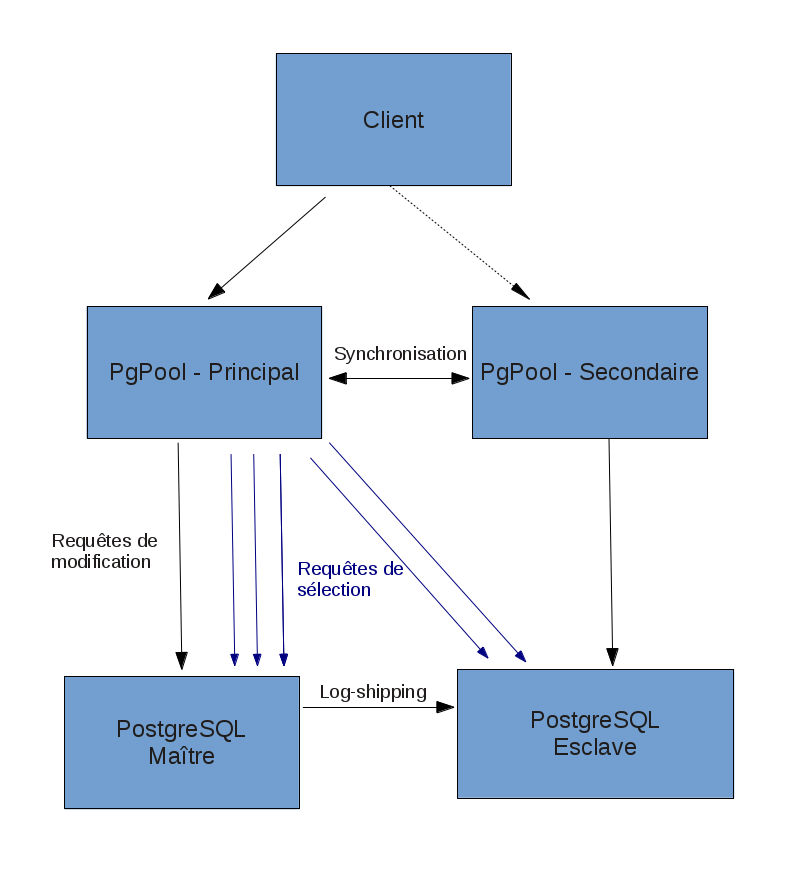
\includegraphics[width=\linewidth]{./arch.png}

Un deuxième serveur esclave a été ajouté en fin de projet afin d'étendre
l'architecture.

\subsection{Configuration}

\subsubsection{Partitionnement}

Pour changer rapidement la configuration de nos architectures au cours des tests,
notre système est en quasi-totalité installé dans un conteneur LVM. Seule la partition 
/boot est en dehors pour simplifier le démarrage.\\


Le conteneur est découpé de façon à accorder 30gb au système hôte, et 30gb par machine
virtuelle. Les systèmes de fichier choisi initialement pour l’ensemble des partitions
au sein du conteneur est l’ext4.\\

\subsubsection{Réseau}

La machine hôte est connectée au réseau au travers d’un bridge br0 au travers d’une
interface physique eth0. Le bridge est présent uniquement en cas de besoin immédiat
et est configuré en IP fixe pour communiquer avec le routeur de la salle.\\

Les machines virtuelles sont quant à elles reliées à l’interface virtuelle virbr0 utilisée
par KVM pour effectuer du NAT. Chaque machine virtuelle dispose de son interface
virtuelle nommé vnetN, connectées par DHCP.\\

\subsubsection{Sécurité}

La sécurité de l'architecture n'étant pas au cœur du sujet, nous avons décidé, comme
pour Bucardo, de ne pas nous préoccuper des problématiques liées. Iptables et
selinux sont donc tout les deux désactivés sur l'ensemble des machines. \\

\subsubsection{Bases de données}

La première étape applicative est le déploiement de bases de données
PostgreSQL. CentOS ne disposant que de la version 8.4, nous avons décidé de
compiler la toute dernière version de PostgreSQL à partir des sources. Quelques
prérequis sont nécessaires pour mener à bien cette compilation : l'installation
de make, gcc, readline-devel et zlib-devel.\\

La configuration des deux serveurs est assez restreinte dans l'ensemble :
adresse et port d'écoute, gestion des logs pour la compatibilité avec les outils
d'analyse. L'ensemble de ces directives sont situées dans le fichier
postgresql.conf (voir annexes). Cependant quelques points doivent être
soulignés :\\

\begin{itemize}
\item wal\_level pour le serveur maître doit être placé à hot\_standby
\item archive\_mode pour le serveur maître doit être activé, l'archive\_command se
doit d'être renseignée
\end{itemize}

Ce dernier point est en effet primordial, c'est ainsi que nous indiquons au
serveur comment stocker les journaux. Dans notre cas, nous allons nous servir de
cette directive pour les placer directement au sein du serveur esclave. C'est à
ce moment là que nous pouvons 

\begin{mVerb}
archive_command = 'scp -o StrictHostKeychecking=no 
    -P PORT_SSH_SLAVE %p PSQL_USER@HOST_SLAVE_IP:PSQL_FOLDER/HOST_MASTER/%f'  
\end{mVerb}

\textit{StrictHostChecking permet d'éviter de vérifier la clé SSH du serveur esclave.} \\


\begin{itemize}
\item pg\_hba.conf doit être correctement renseigné à la fois sur le serveur
esclave et sur le serveur maître afin d'autoriser les connexions entrantes aux
bases de données.\\

\item Depuis la version 9.1, PostgreSQL dispose d'un type de rôle permettant
d'autoriser uniquement la réplication de logs : REPLICATION. Un utilisateur est
donc créé pour permettre ce type d'opérations.\\

\item Du côté esclave, le placement d'un fichier recovery.conf (voir annexes) où
seront écrites les directives nécessaires pour lire les fichiers WAL disposés
précédemment par le serveurs maître (WAL shipping) et les informations de
connexion vers le serveurs maître afin d'obtenir à la source les journaux de
modification (streaming replication). \\
\end{itemize}

Par le biais de ces configurations, nous obtenons la première partie de notre
architecture : deux serveurs PostgreSQL. Le serveur esclave est dès à présent en
mesure de répondre à des requêtes read-only. \\

\subsubsection{pgPool}

De la même façon que PostgreSQL, pour obtenir les dernières fonctionnalités de
pgPool, nous compilerons la version la plus récente disponible. Pour cela,
pgPool a besoin les librairies de développement de PostgreSQL. Nous les
obtiendrons depuis les sources précédentes. De cette façon, nous nous assurons
la compatibilité complète entre tout les acteurs de l'architecture déployée. \\

La configuration se fait au sein du fichier pgpool.conf (voir annexe). PgPool se
comportera en tant que serveur PostgreSQL, il dispose donc d'un port (par défaut
9999) et d'une adresse d'écoute à préciser.\\

Les deux serveurs sont à préciser en plus d'informations telles que le poids
pour le load balancing ou bien si on accepte, ou non, le défaillance d'un des
serveurs. \\

Le mode utilisé dans notre solution est le « master/slave », nous ne renseignons
donc pas les options liées au mode « replication » qui n'est pas compatible avec
celui utilisé actuellement. La directive qui exploite le cœur de l'architecture est «
  master\_slave\_sub\_mode » qui doit être placée à « stream ». \\

Des configurations secondaires peuvent être effectuées pour approfondir le
clustering :\\


\begin{itemize}
\item Le parrallel-mode permettant de spécifier un second serveur pgPool qui sera
configuré exactement de la même façon.\\

\item La gestion du failover et du failback : chaque directive contient l'emplacement
d'un script et des arguments à lui transmettre pour faire basculer le serveur
esclave en serveur maître.\\

\item La vérification du bon fonctionnement de la réplication par pgPool. Il est en
effet en mesure de se connecter directement sur le serveur maître avec les
droits REPLICATION et déclencher un script en cas d'échec.\\

\item L'activation et le dimensionnement du pooling de connexions.\\
\end{itemize}

La dernière étape est le lancement des trois serveurs.

\begin{mVerb}
[root@vm2 ~]# su - postgres -c '/srv/psql/bin/pg_ctl -D /srv/psql/data/ start'
server starting
\end{mVerb}

\begin{mVerb}
[root@vm3 ~]# su - postgres -c '/srv/psql/bin/pg_ctl -D /srv/psql/data/ start'
server starting
\end{mVerb}

\begin{mVerb}
[root@vm1 pgpool]# pwd
/srv/pgpool
[root@vm1 pgpool]# ./bin/pgpool 
[root@vm1 pgpool]#
\end{mVerb}

\subsection{Vérifications de l'architecture et tests de fonctionnement}

Dans un premier temps, il nous faut vérifier le bon fonctionnement de la
réplication entre le maître et l'esclave. Pour cela, nous nous connectons
naturellement sur le serveur maître et effectuons une opération d'écriture.

\begin{mVerb}
[root@vm2 psql]# ./bin/psql -U postgres 
psql (9.2.3)
Type "help" for help.

postgres=# create database test2;
CREATE DATABASE
postgres=# \l
                                  List of databases
   Name    |  Owner   | Encoding |   Collate   |    Ctype    |   Access privileges   
-----------+----------+----------+-------------+-------------+-----------------------
 pgpool    | postgres | UTF8     | en_US.UTF-8 | en_US.UTF-8 | 
 postgres  | postgres | UTF8     | en_US.UTF-8 | en_US.UTF-8 | 
 template0 | postgres | UTF8     | en_US.UTF-8 | en_US.UTF-8 | =c/postgres          +
           |          |          |             |             | postgres=CTc/postgres
 template1 | postgres | UTF8     | en_US.UTF-8 | en_US.UTF-8 | =c/postgres          +
           |          |          |             |             | postgres=CTc/postgres
 test1     | postgres | UTF8     | en_US.UTF-8 | en_US.UTF-8 | 
 test2     | postgres | UTF8     | en_US.UTF-8 | en_US.UTF-8 | 
(6 rows)
\end{mVerb}


Nous pouvons ensuite vérifier que l'opération s'est bien répliquée sur le
serveur esclave : \\

\begin{mVerb}
[root@vm3 ~]# /srv/psql/bin/psql -U postgres -p 5433
psql (9.2.3)
Type "help" for help.

postgres=# \l
                                  List of databases
   Name    |  Owner   | Encoding |   Collate   |    Ctype    |   Access privileges   
-----------+----------+----------+-------------+-------------+-----------------------
 pgpool    | postgres | UTF8     | en_US.UTF-8 | en_US.UTF-8 | 
 postgres  | postgres | UTF8     | en_US.UTF-8 | en_US.UTF-8 | 
 template0 | postgres | UTF8     | en_US.UTF-8 | en_US.UTF-8 | =c/postgres          +
           |          |          |             |             | postgres=CTc/postgres
 template1 | postgres | UTF8     | en_US.UTF-8 | en_US.UTF-8 | =c/postgres          +
           |          |          |             |             | postgres=CTc/postgres
 test1     | postgres | UTF8     | en_US.UTF-8 | en_US.UTF-8 | 
 test2     | postgres | UTF8     | en_US.UTF-8 | en_US.UTF-8 | 
(6 rows)
\end{mVerb}

Nous pouvons par la même occasion constater que le serveur esclave n'est
accessible qu'en lecture. Si nous tentons une écriture nous obtenons le message
suivant : \\

\begin{mVerb}
postgres=# create database toto;
ERROR:  cannot execute CREATE DATABASE in a read-only transaction
\end{mVerb}
 

La prochaine étape est de contrôler que pgPool est bien déployé. Nous effectuons
le même type de vérification sommaires.

\begin{mVerb}
[root@vm1 ~]# /srv/psql/bin/psql -U postgres -p 9999
psql (9.2.3)
Type "help" for help.

postgres=# \l
                                  List of databases
   Name    |  Owner   | Encoding |   Collate   |    Ctype    |   Access privileges   
-----------+----------+----------+-------------+-------------+-----------------------
 pgpool    | postgres | UTF8     | en_US.UTF-8 | en_US.UTF-8 | 
 postgres  | postgres | UTF8     | en_US.UTF-8 | en_US.UTF-8 | 
 template0 | postgres | UTF8     | en_US.UTF-8 | en_US.UTF-8 | =c/postgres          +
           |          |          |             |             | postgres=CTc/postgres
 template1 | postgres | UTF8     | en_US.UTF-8 | en_US.UTF-8 | =c/postgres          +
           |          |          |             |             | postgres=CTc/postgres
 test1     | postgres | UTF8     | en_US.UTF-8 | en_US.UTF-8 | 
 test2     | postgres | UTF8     | en_US.UTF-8 | en_US.UTF-8 | 
(6 rows)
\end{mVerb}

\begin{mVerb}
postgres=# create database test3;
CREATE DATABASE
postgres=# \l
                                  List of databases
   Name    |  Owner   | Encoding |   Collate   |    Ctype    |   Access privileges   
-----------+----------+----------+-------------+-------------+-----------------------
 pgpool    | postgres | UTF8     | en_US.UTF-8 | en_US.UTF-8 | 
 postgres  | postgres | UTF8     | en_US.UTF-8 | en_US.UTF-8 | 
 template0 | postgres | UTF8     | en_US.UTF-8 | en_US.UTF-8 | =c/postgres          +
           |          |          |             |             | postgres=CTc/postgres
 template1 | postgres | UTF8     | en_US.UTF-8 | en_US.UTF-8 | =c/postgres          +
           |          |          |             |             | postgres=CTc/postgres
 test1     | postgres | UTF8     | en_US.UTF-8 | en_US.UTF-8 | 
 test2     | postgres | UTF8     | en_US.UTF-8 | en_US.UTF-8 | 
 test3     | postgres | UTF8     | en_US.UTF-8 | en_US.UTF-8 | 
(7 rows)
\end{mVerb}

La création réussie d'une base de données prouve bien que pgPool est mesure
d'effectuer ses requêtes d'écriture sur la bonne base de donnée. En effet, pour
déterminer quelle DB est maître il effectue la requête suivante à la fois au
démarrage de pgPool et régulièrement pendant son fonctionnement :
\\

\begin{mVerb}
2013-03-25 00:59:11 DEBUG: pid 12165: do_query: extended:0 query:SELECT pg_is_in_recovery()
\end{mVerb}

Cette requête selon le serveur retourne un résultat différent selon le type de
serveur. Sur le serveur esclave nous obtenons : \\

\begin{mVerb}
[root@vm3 ~]# /srv/psql/bin/psql -U postgres -p 5433
psql (9.2.3)
Type "help" for help.

postgres=# SELECT pg_is_in_recovery();
 pg_is_in_recovery 
-------------------
 t
(1 row)
\end{mVerb}

Et sur le serveur maître nous obtenons : \\

\begin{mVerb}
[root@vm2 ~]# /srv/psql/bin/psql -U postgres
psql (9.2.3)
Type "help" for help.

postgres=# SELECT pg_is_in_recovery();
 pg_is_in_recovery 
-------------------
 f
(1 row)
\end{mVerb}

\subsubsection{L'état du clustering avec PCP}

pgPool permet facilement de s'interfacer avec des scripts écrits par
d'administrateur grâce à une micro-API. Nous disposons en effet de quelques
commandes pour connaître l'état de chaque nœud, attacher ou détacher des nœuds
à la volée ou encore obtenir l'état des processus de pgPool. Ci-dessous quelque
exemples d'utilisation… \\

\begin{mVerb}
[root@vm1 pgpool]# ./bin/pcp_node_info 5 localhost 9998 pgpool test 0
10.1.0.2 5432 1 0.500000
[root@vm1 pgpool]# ./bin/pcp_node_info 5 localhost 9998 pgpool test 1
10.1.0.3 5433 1 0.500000 
IP      PORT ETAT POIDS

[root@vm1 pgpool]# ./bin/pcp_node_count 5 localhost 9998 pgpool test
2

[root@vm1 pgpool]# ./bin/pcp_proc_count 5 localhost 9998 pgpool test
12607 12608 12609 12610 12611 12612 12613 12614 12615 12616 12617 12618 12619
12620 12621 12622 12623 12624 12625 12626 12627 12628 12629 12630 12631 12632
12633 12634 12635 12636 12637 12638 12639 12640 12641 12642 12643 12644 12645
12646 12647 12648 12649 12650 12651 12652 12653 12654 12655 12656 … … … … …
\end{mVerb}

La dernière commande utilisée est évocatrice de la façon dont pgPool est
conçu. Il lance en effet \textit{num\_init\_children} processus, appelés « pool
» (ici 400, par défaut 32) qui seront en mesure de supporter \textit{max\_pool}
(par défaut 4) connexions par pool.

\subsection{Test de performances}

Le plus gros problème rencontré lors de notre projet a été la difficulté de
prouver que pgPool apportait une valeur ajoutée à nos architectures. En effet,
malgré un clustering favorable à des requêtes en lecture seule (notre serveur
esclave est mesure de traiter 50\% des requêtes), nous avons obtenu des
résultats largement inférieurs lors de tirs sur le serveur pgPool que sur un des
deux serveurs PostgreSQL. \\

\textit{Tir composé de SELECT, sans nettoyage de Vacuum (requête d'écriture qui ne
serait pas redirigée vers le serveur esclave), 50 clients, 10 secondes.} \\

\begin{mVerb}
[root@projet-clustering ~]# /srv/psql/bin/pgbench -U postgres -p 5432 -h vm2 -T
10 -S -n -c 50 test1

transaction type: SELECT only
scaling factor: 1
query mode: simple
number of clients: 50
number of threads: 1
duration: 10 s
number of transactions actually processed: 29103
tps = 2884.297767 (including connections establishing)
tps = 3024.772516 (excluding connections establishing)
\end{mVerb}

pgPool étant composé d'un grand nombre d'options, nous avons pu appuyer sur
différents leviers pour orienter les chiffres en notre faveur. Activation ou
désactivation du pooling, du load balancing, changement des poids des serveurs,
logs, réplication des connexions… Sans grands résultats…\\

La situation ne s'est débloquée que tardivement. Nos solutions de tests ne
disposaient en effet que de peu de performances, limitant fortement les
possibilités de pgPool. Nous avons pris la décision de louer des serveurs plus
performants pendant quelques heures pour déployer nos architectures dans des
conditions plus réalistes. \\

En poussant jusqu'au boût les compostants du cluster de serveurs, nous avons pu
obtenir des chiffres convaincants. Nous avons dû également augmenter le nombre
de serveurs esclaves à deux, pour augmenter les bénéfices du load balancing en
SELECT only. L'utilisation du cache mémoire intégré à pgBench a également permit
d'améliorer grandement la situation. \\

Le contenu détaillé de nos tests est situé en annexes E.

\subsection{Échecs}

\subsubsection{Mode parallèle}

Comme précisé plus haut, le déploiement d'une seconde instance d'un serveur de
pgPool a échoué. Les étapes pour sa configuration sont la création d'une base de
données pgPool qui sera inclue au sein du clustering et qui servira de stockage
des informations de l'état des nœuds à des fins de synchronisation. La
difficulté importante pour vérifier les échanges entre les deux serveurs pgPool
nous aura mis en échec. \\

\subsubsection{Fail-over}

Le fail-over de pgPool aura été également un échec partiel, en grande partie liée au
manque de temps. PgPool dispose en effet d'un vaste panel de variables que nous
pouvons transmettre au script de fail-over. Ce script doit être chargé de
placer sur le serveur esclave un fichier (dont nous déterminerons le nom dans
son \textit{recovery.conf}), qui lorsque le dernier le détectera, basculera
automatiquement en mode de lecture/écriture, pouvant ainsi remplacer le
maître. \\

\begin{mVerb}
trigger_file = '/srv/psql/data/trigger'
\end{mVerb}

Nous détaillerons tout de même la procédure manuelle, sans grande utilité… \\

Vérification que le serveur esclave est bien esclave :\\

\begin{mVerb}
[root@vm3 data]# /srv/psql/bin/psql -U postgres -p 5433
psql (9.2.3)
Type "help" for help.

postgres=# create database test3;
ERROR:  cannot execute CREATE DATABASE in a read-only transaction
\end{mVerb}

Arrêt du serveur maître : \\

\begin{mVerb}
[root@vm2 psql]# su - postgres -c '/srv/psql/bin/pg_ctl -D /srv/psql/data/ -m immediate stop'
waiting for server to shut down.... done
server stopped
\end{mVerb}

Bascule du serveur esclave : \\

\begin{mVerb}
[root@vm3 data]# touch trigger
\end{mVerb}

Vérification d'écriture :\\

\begin{mVerb}
[root@vm3 data]# /srv/psql/bin/psql -U postgres -p 5433
psql (9.2.3)
Type "help" for help.

postgres=# create database test4;
ERROR:  cannot execute CREATE DATABASE in a read-only transaction
postgres=# create database test4;
CREATE DATABASE
postgres=# 
\end{mVerb}

Des tests ont été effectués avec succès lorsque ce fichier est placé « à la main
», cependant pgPool n'a jamais été en mesure de déclencher ce script au bon
moment. Avec un peu plus de persévérence peut-être que… \\

\section{Comparatif des solutions}

L'architecture de PgPool est moins ambitieuse que celle déployée avec Bucardo :
nous ne traitons pas la synchronisation maître maître. En échange d’un ensemble
de fonctionnalités moins complet, nous obtenons une solution plus robuste et
plus fiable. Nous n’avons pas à nous préoccuper des possibles problèmes de
requêtes concurrentes, mais Bucardo sait gérer les problèmes de conflits
d'écriture. Mais quand bien même Bucardo sait exploiter un cluster de type
actif/actif, il se limite à deux nœuds uniquement.\\

L’utilisation de la réplication native à PostgreSQL est également un gage de
stabilité et de performance : en effet, moins de tâches sont déléguées à des
acteurs extérieurs, ce qui n'est pas le cas de Bucardo qui s'appuie sur des
démons écrits en perl, pas forcément réputé pour sa rapidité. En revanche,
Bucardo bénéficie d'une simplicité dans sa mise en œuvre depuis le shell, grâce
précisément à l'usage des commandes externes.\\

En outre, Bucardo ne sait pas gérer la réplication de DDL, tandis que PgPool
lui, sait répliquer aussi les requêtes de définitions de données.\\


PgPool au final, ne dispose pas d’un rôle très vaste et se limite à la gestion
de connexions. Bucardo va plus loin puisqu'il maintient par le biais de driver
perl spécifique à Postgresql, l'organisation de sa propre base de données,
destinée à la gestion des modifications apportées dans les lignes des tables
impliquées dans les set de réplication.\\

PgPool, au même titre que PostgreSQL, dispose d’un fonctionnement proche de la
philosophie UNIX. Beaucoup de fonctionnalités doivent être configurées via des
scripts, rendant la tâche de l’administrateur plus longue. La fiabilité des
solutions de failover repose donc en partie sur la rigueur consacrée dans
l’écriture des scripts liés à ces tâches. En compensation, nous gagnons ainsi en
liberté.\\

Pour répartir les requêtes, pgPool va devoir en connaître le coeur, et donc les
analyser pour différencier les requêtes modificatrices des requêtes de
sélection. À la manière du modèle OSI, interagir au niveau de cette couche
applicative est coûteux en performances. Bucardo, dans sa configuration maître
esclave, ne permet pas le mode hot-standby comme PgPool, et ne peut donc pas
utiliser le serveur esclave en lecture seule.\\

Ainsi, en plus de PostgreSQL c’est donc un tout nouveau logiciel qu’il va
falloir sans cesse optimiser selon ses besoins. PgPool dispose en effet d’un
grand nombre de paramètres à régler tels que la configuration du pooling ou bien
celles du cache mémoire. En revanche, Bucardo n'est pas prévu pour proposer du
pooling de connexions.\\

Si nous souhaitons utiliser le log shipping, nous avons de forts prérequis de
versions : il nous faudra au minimum la version 9.0 de PostgreSQL pour
bénéficier de cette fonctionnalité. Certaines distributions « stables » du
moment sont donc concernées par ce problème telle que Debian Squeeze qui ne
dispose que de la version 8.4. Sortir du système de paquets de son système est
donc à envisager. Bucardo est beaucoup moins contraint en terme de version,
mieux encore, avec Bucardo, on peut même envisager d'effectuer de la migration
de base d'une version 8.x à 8.y, d'un os vers un autre, pourquoi pas, il suffit
pour cela de créer un 'sync' de type 'fullcopy' ou 'pushdelta' en mode
'onetimecopy=2'.\\

PgPool est un SPOF sans le mode parallèle, il faudra donc veiller à ce qu'un
autre service PgPool existe sur une autre machine et à mettre en place un
mécanisme de basculement comme heartbeat ou lvs. Bucardo, par défaut, n'est pas
sujet à cette faiblesse.\\

PgPool est donc basé sur de la réplication de requêtes SQL, il faut donc veiller
à ce que les bases de données ne soient accessibles que via PgPool, et non
directement, au risque de désynchroniser les clusters. Bucardo ne souffre pas de
cette limitation vu qu'il travaille au niveau de la ligne par le biais de
trigger, et qu'il contrôle lui-même les modifications à propager.\\

Enfin, Bucardo, en standard, ne sait pas faire de redondance de charge, tandis
que PgPool intègre cette fonctionnalité. Mais certaines limites de Bucardo
peuvent être facilement compensées par l'usage de produits tiers comme pgbouncer
pour faire du pooling de connexions, ou bien haproxy pour proposer de la
redondance de charge.\\


\chapter{Quelques repères de comparaison}

\section{Présentation des produits de clustering Oracle DataGuard et Oracle RAC}

\subsection{Base de données Oracle et Oracle Data Guard}

Oracle Data Guard est une solution de haute disponibilité (High Availability –
HA) et de restitution de données après sinistre (Disaster Recovery – DR) qui
fournit des mécanismes automatisés et ultra-rapides de recouvrement d'incidents,
qu'il s'agisse d'anomalies du SGBDR lui-même, ou bien de la défaillance ou de la
corruption d'un nœud du système. De plus, la base de données dite standby (celle
sur laquelle les données sont répliquées) peut malgré tout être utilisée en mode
lecture seule et peut donc répondre à des requêtes de lecture de différentes
natures, aussi bien pour du reporting que pour des tests de
développement. Oracle Data Guard est disponible en standard dans la version
Enterprise d'Oracle RDBMS. \\

Voici d'ailleurs la configuration typique d'une solution avec Oracle Data
Guard : \\

\begin{center}
  \includegraphics[width=11cm]{15.eps}
\end{center}\\

Quoique les solutions traditionnelles comme la sauvegarde et la restauration
depuis des bandes, ou bien la distribution des données sur des miroirs distants
puissent fournir de bons niveaux de haute disponibilité, Oracle Date Guard
fournit de loin les solutions les plus étendues en matière de haute
disponibilité. \\


Par rapport aux solutions traditionnelles de recouvrements d'incidents, Oracle
Data Guard offre de nombreux avantages, tels que : \\

\begin{itemize}
\item mécanismes automatisés contre la corruption de données dues à des écritures
  perdues ou à bien dues à des défaillances des bases elles-mêmes.
\item système automatique de remplacement de blocs de données corrompues sur le
  serveur primaire ou sur le serveur standby (en mode physique) depuis un serveur
  physique « standby » ou bien depuis le serveur primaire.
\item Protections étendues contre la perte de données sur le serveur primaire.
\item temps de basculement en vue de la sauvegarde ou de la migration de données
  bien plus réduit en utilisant Data Guard Switchover.
\item temps d'actualisation des actions d'actualisation menées par Data Guard
  sensiblement réduit.
\item aptitudes à délester le serveur primaire de certaines activités comme le
  backup, la gestion des requêtes ou bien encore le reporting grâce à
  l'utilisation simultanée du serveur standby en mode read-only, et ce, sans
  pénaliser le bon fonctionnement du primaire.
\item possibilités d'utiliser tout fichier non lié directement à la base de
  données dans le système de fichier spécifique d'Oracle ( Database File System
  - DBFS)
\item pas besoin de redémarrer le système, ou de reconnecter les applications
  clientes ou bien encore de recalibrer les systèmes de sauvegarde après un
  recouvrement après incident.
\item transparence pour les applications
\item transparence et support intégré en cas de défaillance d'applications
\item efficience dans les utilisations réseaux.
\end{itemize}

\vspace{1cm}

De même, pour toutes les données abritées sur une infrastructure basée sur
Oracle RDBMS, Oracle Data Guard qui possède la fonction intégrée « zero-data
  loss », est bien plus efficace, bien mieux optimisé contre la perte de données
que les traditionnelles solutions en miroir, voici d'ailleurs les principaux
avantages de Data Guard : \\

\begin{itemize}
\item Meilleure efficience réseau car seuls les « redo data » ont besoin d'être
expédiés sur le site distant, et de plus, elles peuvent être compressées, alors
que dans le cas d'une solution de mirroring, les fichiers de données doivent
être transférés, ainsi que les fichiers de redo, et bien d'autres données
encore.

\item Meilleures performances car seules les écritures dans les fichiers de redo sont
transférés, ce qui n'est pas le cas avec les sites mirroirs, où de nombreuses
autres écritures sont nécessaires. En outre, Oracle Data Guard n'affecte en rien
les performances en écriture sur les fichiers de données, puisqu'ils ne
sollicite pas le mécanisme DBWR (Oracle DataBase Writer).

\item Meilleurs protection de données, car en effet, Oracle Data Guard assure une
protection renforcée contre la corruption de données dues à des écritures
erronées sur les disques, à cause de problèmes matériels par exemple, étant
donné que ne sont sauvegardés que les fichiers de redo, dont la consistence est
vérifiée, ce qui n'est pas le cas des solutions miroirs qui propagent les
anomalies.

\item Grande flexibilité dans la mise en œuvre d'Oracle Data Guard compte tenu qu'une
simple liaison réseau TCP/IP suffit, et il n'est nul besoin de matériels
supplémentaires couteux.

\item Oracle Data Guard offre de nombreuses fonctionnalités étendues et des solutions
performantes pour la protection de données, comme par exemple Active Data Guard,
les « redo apply » pour les serveurs en mode standby physique, ou encore les
« sql applay » pour les serveur en mode standby logique, mais aussi des
mécanismes automatiques en mode « push-button » de basculement vers un état
stable et fonctionnel, pour des rôles dits « switchover » ou « failover », sans
oublier des outils d'administration et de monitoring en mode graphique.
\end{itemize}

\vspace{1cm}

Afin d'illustrer les deux modes de fonctionnement principaux de Data Guard,
voici deux représentations typiques, tout d'abord Data Guard en mode standby
physique : \\

\begin{center}
  \includegraphics[width=12cm]{16.eps}
\end{center}\\

Puis vient la solution en mode standby logique : \\

\begin{center}
  \includegraphics[width=14cm]{17.eps}
\end{center}\\

Avant d'aller plus loin, et juste pour fixer les idées, les redo log sont des
fichiers, créés pour chaque instance de la base de données Oracle, qui
enregistrent tous les changements ayant été initiés sur le SGBD, et selon une
procédure bien déterminée, afin d'éviter la perte de données et la corruptions
de ces dernières. \\

Les fichiers de redo sont au nombre de deux minimum, et sont complétés selon un
mécanisme de permutation circulaire, ainsi que le montre le graphique suivant : \\

\begin{center}
  \includegraphics[width=8cm]{18.eps}
\end{center}\\

Il n'y a qu'un seul fichier courant à la fois, celui sur lequel doit s'effectuer
l'écriture des changements effectués sur la base de données, mais il y a aussi
un fichier de redo actif, celui sur lequel peut s'effectuer une opération de
récupération de données, et enfin les fichiers de redo inactifs sur lesquels la
récupération des données a déjà été traitée. \\

Classiquement, une base de données Oracle fonctionne donc selon l'un des deux
modes, aussi appelés des rôles, à savoir le fonctionnement en serveur primaire
ou en serveur standby. Ainsi, lorsque l'on utilise Data Guard, il est possible
de passer d'un rôle à l'autre, soit avec la méthode dite « switchover », soit
avec la méthode « failover ». \\

La méthode « switchover » consiste à basculer, sans perte de données, le
fonctionnement de la base de données vers l'un des serveurs en mode standby, la
plupart du temps à des fins de maintenance sur le serveur primaire, puis à
repasser le SGBD en production normale sur le serveur primaire une fois les
opérations de maintenance réalisées sur ce dernier. \\

Quant à la méthode « failover », sa mise en œuvre a lieu précisément lorsqu'une
anomalie du serveur primaire survient, à ce moment là, le serveur standby
endosse le rôle de serveur primaire. Les administrateurs de la base peuvent
évidemment configurer ce rôle, de telle façon qu'il n'y ait  aucune perte de
données. \\

Ces transitions de rôles peuvent éventuellement être implémentées par le biais
de requêtes SQL, mais elles peuvent aussi être automatisées grâce au « Data
  Guard Broker » que nous allons expliquer succinctement ci-après. \\

\subsubsection{Oracle Data Guard et le Data Guard Broker}

Le Data Guard Broker est en fait un espace fonctionnel distribué, regroupant à
la fois le serveur primaire et les serveurs standby, qu'ils soient éparpillés
géographiquement ou non, permettant l'automatisation et la centralisation de la
création, la maintenance et le monitoring des configurations de Data Guard. Que
ce soit en mode GUI avec Oracle Enterprise Manager, ou en mode CLI avec le
DGMGRL, voici ce que permet ce « broker » :


\begin{itemize}
\item Création et activation des configurations Data Guard, incluant la mise en
  place des services  de redo.

\item Administration de l'intégralité des configurations de Data Guard depuis
  n'importe quel système.

\item Administration et surveillance des configurations de Data Guard, contenant
  à la fois des serveurs standby, mais aussi des serveurs primaires sur une
  architecture Oracle Real Application Cluster (RAC)

\item Simplification de la mise en œuvre des mécanismes de « switchover » ou de
  « failover » par un simple clic ou une simple ligne de commande.

\item Automatisation d'un basculement rapide vers le serveur standby désigné en
  cas d'anomalies sur le serveur primaire, sans intervention d'un DBA.
\end{itemize}

\vspace{1cm}

Voici le schéma général du positionnement dans le système du Data Guard Broker :
\\

\begin{center}
  \includegraphics[width=10cm]{19.eps}
\end{center}\\

En outre, Oracle Enterprise Manager automatise et simplifie :

\begin{itemize}
\item Création d'un serveur standby en mode physique ou logique à partir d'une
sauvegarde du serveur primaire.

\item Ajout à une configuraiton Data Guard d'un serveur standby nouveau ou
  existant.

\item Surveillance des logs, capture des informations de diagnostic et détection
rapide des problèmes grâce aux outils inclus de tests, de performances et de
monitoring.
\end{itemize}
\vspace{1cm}

Pour finir, voici un récapitulatif des différents composants du Data Guard
Broker et des relations entre les objets, le tout en image :

\begin{center}
  \includegraphics[width=13cm]{20.eps}
\end{center}\\

\subsection{Oracle RAC}

\subsubsection{Clusters Oracle}

Oracle RAC ( Real Application Cluster ) est un système de gestion de bases de
données relationnelles. \\

La particularité de l’option RAC d’Oracle Enterprise est d’accroitre la haute
disponibilité et l’extensibilité de la base de données. Cela permet d’apporter
une réponse à l’augmentation rapide et continue du volume de données ainsi
qu’aux exigences de haute performance. \\

Oracle RAC se base sur le concept de cluster et utilise donc une approche de
déploiement horizontale (scale-out) qui permet d’augmenter la puissance de
calcul totale du cluster en augmentant le nombre de serveurs. \\

En effet, de nos jours une base de données doit être accessible en permanence et
peut rarement supporter la moindre immobilisation même à des fins de maintenance
ou lors de défaillance. \\

\subsubsection{Architecture RAC}

Une implémentation RAC typique regroupe de nombreuses instances Oracle
s'éxécutant sur de nombreuses machines, ou neuds. Ces noeuds communiquent entre
eux et partagent un pool commun tous des fichiers de données de la base. \\

	Chaque noeud est reliés aux autre grâce à une collectivité à haut débit.
Chaque noeud dispose de ses propres fichier redo (Ces fichiers contiennent
l'historique des modifications effectuées sur la base de données ).\\

Le gestionnaire de cluster surveille l'état de chaque instance de base de
données dans le cluster et leur permets de communiquer entre elles. Il est aussi
appelé Cluster Synchronization Service (CSS).\\

Le service cache global (global cache service) contrôle l'échange de données
entre les noeuds en utilisant la technologie Cache Fusion. Celle-ci synchronise
le cache mémoire de tous les noeuds via des connexions rapides, autorisant
chacun à accéder à n'importe quelles données stocké dans la base.\\

Le stockage partagé (shared storage) consiste en des fichiers de données et
d'index ainsi qu'en des fichiers de contrôle.\\

Cette architecture permet aux système RAC d'être hautement disponible.
Par exemple si un noeud est défaillant ou nécessite une maintenance, les autres
noeuds vont assurer l'accès à la base. Tout cela est transparent pour
l'utilisateur ou l'application dés lors qu'au moins un noeud reste actif. \\

RAC offre une évolutivité presque linéaire et conduit à une augmentation des
performances. Des noeuds peuvent être facilement ajouté aux cluster lorsque cela
est nécessaire pour faire face à un accroissement de l'activité. \\

\subsubsection{Oracle Database avec Oracle One Node}

Traditionnellement Oracle RAC a était conçu pour une architecture multi-noeuds
c'est-à-dire une base de données qui fonctionne sur plusieurs serveurs. Oracle
RAC one node comme son nom l'indique permets de faire fonctionner la base de
données que sur un seul noeud du cluster.  \\

Ainsi, cette fonction permets de consolider toutes les base de données en un
seul cluster pour faciliter la gestion, toute en offrant une haute disponibilité
car en canne de panne la base est automatiquement activée sur un autre
serveur. Si le noeud est surchargé, on peut déplacer l'instance vers un autre
noeud du cluster en utilisant le transfert en ligne de la base sans interruption
pour les utilisateurs. \\


On peut allouer des ressources du serveur à l'aide de Oracle Database Resource
Manager Instance Caging. L'evolutivité du serveur est illimité, en effet si les
application se developpe et exige plus de ressource que un noeud ne peut
fournir, on peut effectuer une mise à niveau en ligne et revenir à la
traditionnel configuration multi-noeuds d'Oracle RAC. \\

Les avantages de haute disponibilité de Oracle RAC One Node sont : \\

\begin{itemize}
\item Offre une meilleure disponibilité de bases de données pour le basculement
  à  froid.
\item Offre une meilleure virtualisation des bases des données que les solution
  baser sur l'hyperviseur.
\item Permet la migration, correction en ligne et mise à niveau du système
  d'exploitation et des logiciels de la base.
\item Offre une approche global d'une solution d'un fourniseur unique sans qu'il
  soit nécessaire de mettre en œuvre des produits tiers.
\item On peut passer à Oracle RAC avec la configuration multi-noeuds.
\item Fournit un environnement standardiser et un ensemble d'outils commun pour
  les déploient à nœud unique et multi-noeuds de base Oracle.
\item Est moins chère que les solution Oracle RAC
\item Compatible avec Oracle Dataguard. Toute base de données dans une
  configuration Dataguard, si une base de données primaire ou de
  secours,peut-être une base de donnée Oracle One Node.
\end{itemize}
\vspace{1cm}

	Pour la virtualisation, quand on utilise Oracle RAC One Node avec Oracle VM on
  augmente la haute disponibilité et l'évolutivité d'Oracle RAC. Si les capacité
  de la VM  sont trop faible, on peut migrer l'instance Oracle RAC One  vers un
  autre nœud Oracle VM plus importants dans le groupe ou déplacer l'instance
  Oracle RAC One vers un autre nœud Oracle VM, puis redimensionner la VM
  d'Oracle. Lorsqu'on déplace l'instance Oracle RAC One Node on doit à nouveau
  redimensionner la VM d'Oracle on peut augmenter dynamiquement les limite
  programmé avec Ressource Manager Instance Caging.

\subsubsection{Oracle Database avec Oracle RAC}

Une architecture Oracle Database avec Oracle RAC est en soi un systéme à haute
disponibilité. Contrairement à un serveur de base de données monolithique
traditionnelle qui coûte chére et c'est capacite de changement ne sont pas
flexible et on bessoin de beaucoup de ressources, Oracle RAC combine la
puissance de traitement de plusieurs ordinateurs reliés entre eux pour assurer
la redondance du système,  évolutivité, et la haute disponibilité. \\

Les clusters qui sont typiques des environnements Oracle RAC peut fournir un
service continu pour des arrêts prévus et imprévus. Oracle RAC a des niveau de
disponibilité supérieur aux fonction standart d'Oracle Database. Toutes les
fonctions d'instance unique de haute disponibilité telles que les technologies
de Flashback et la réorganisation en ligne, s'appliquent également à Oracle
RAC. Applications scale dans Oracle RAC permet de répondre à la demande
croissante de traitement des données sans modifier le code de l'application. En
outre cela permet d'effectuer des opération de maintenance sur un sous-ensemble
des composants du cluster  alors que l'application continue de tourner sur le
reste du cluster cela permet de réduire les temps d'arrêt planifié. \\


Oracle RAC exploite la redondance qui est fourni par le cluster afin d'assurer
une disponibilité à n-1 nœuds défaillants dans un cluster de n
nœuds. Contrairement au modèle de cluster actif/passif où un nœud est
complètement inactif, toutes les instances et les nœuds peuvent être actives à
l'échelle de votre application. La communication entre les nœuds est optimisé
par le biais de l'interconnexion redondante d'utilisation (sans nécessiter
l'utilisation d'un cautionnement ou d'autres technologies) pour assurer la
stabilité, la fiabilité et l'évolutivité.\\
 

Oracle Database avec l'architecture Oracle RAC offre les avantages suivants par
rapport à un serveur de base de données monolithique traditionnel et le modèle
de cluster de basculement à froid : \\

\begin{itemize}
\item Évolutivité à travers les base de données.
\item Possibilité d'augmenter la capacité de traitement sans interruption ou
modification de l'application
\item Capacités à tolérer et à rapidement récupérer d'une panne informatique.
\item Optimisé communication du cluster via des interfaces réseau redondantes,
  sans utiliser de liaison ou d'autre technologies
\item Mises à jour dangereuse pour les modifications du système et le changement
  de matériel.
\item Mises à jour de patch  pour certains correctifs provisoires, des
  correctifs de sécurité, les processeurs et les logiciels du cluster 
\item Rapide, automatique et connexion intelligente et service de relocalisation
  et basculement.
\item Gestion globale intégrant les fonctionnalité de base et gestion
  caractéristique du cluster basé sur Grid Plug and Play.
\item Load balancing de conseil et d'exécution de l'aide équilibrage de charge
  de connexion réorienter et équilibrer le travail entre les ressources
  appropriées. 
\item Oracle Quality of Service (QoS) pour la gestion basée sur les stratégies
  d'exécution de gestion de l'allocation des ressources de bases de données aux
  charges de travail pour assurer des niveaux de service sont respectés dans
  l'ordre des besoins de l'entreprise dans des conditions dynamiques. 
\item Oracle Enterprise Management support pour  Oracle ASM and Oracle ACFS, Grid Plug
and Play, Cluster Resource Management, Oracle Clusterware and Oracle RAC
Provisioning and patching.
\end{itemize}
\vspace{1cm}

\begin{center}
  \includegraphics[width=10cm]{21.eps}
\end{center}\\

\subsubsection{Oracle Database avec Oracle RAC sur clusters étendues}

Oracle Database avec l'architecture Oracle RAC est connue avant tout comme pour
sont évolutivité et sa haute disponibilité qui réside dans un centre de données
unique. Il est possible, dans certaines circonstances, de construire et de
déployer un système d'Oracle RAC où les nœuds du cluster sont séparés par de
grandes distances. Cette architecture est considéré comme un cluster étendu. \\ 


Un cluster Oracle RAC étendue est une architecture qui permet une récupération
très rapide de panne du site et permet à tous les nœuds, à tous les sites à
traiter activement les opérations dans le cadre du cluster de base de données
unique. Par exemple, pour une entreprise qui a un campus d'entreprise, la
configuration de l'extension Oracle RAC peut consister en différents nœuds
Oracle RAC situés dans des bâtiments séparés. Le cluster Oracle RAC étendue
offre la haute disponibilité d'un cluster Oracle mais ne peut pas répondre aux
éxigence de panne d'un cluster RAC. \\


Lorsque les deux centres de données sont situés relativement proches les uns des
autres,  les clusters étendue peuvent fournir une excellente protection pour
certaines catastrophes, mais pas tous. Vous devez déterminer si les deux sites
sont susceptibles d'être touchés par la même catastrophe. Par exemple, si la
configuration du cluster étendu est correctement configuré, il peut protéger
contre les catastrophes comme une panne d'électricité locale, un accident
d'avion, ou une salle de serveur inondée. Cependant, un cluster étendu ne peut
pas protéger contre toutes les corruptions de données ou de données spécifiques
échecs qui influent sur la base de données, ou contre les catastrophes globales,
telles que les tremblements de terre, les ouragans, les inondations et
régionales qui affectent une plus grande zone géographique. \\


Les avantages de l'utilisation d'Oracle RAC sur les clusters étendus : \\

\begin{itemize}
\item Aptitude à utiliser toutes les ressources du système sans mettre en péril
  les temps de basculement global des défaillances d'instance et nœud.
\item Récupération rapide si un site tombe en panne.
\item Tous les avantages énumérés Oracle RAC 
\end{itemize}


\chapter*{Conclusion}
\addcontentsline{toc}{chapter}{Conclusion}

Le « libre » permet de déployer des solutions de clustering et de HA de bonne
tenue mais n'a pas l'aura marketing et commerciale des leaders du
marché. Alors, comment pourrions-nous le promouvoir ?\\

Tout d'abord, ça commence ici à Nancy, à l'IUT Charlemagne puisque nous avons eu
la chance d'être sélectionnés pour suivre la licence pro ASRALL, qui permet un
large tout d'horizon du monde du libre, et qui permet notamment par le biais du
projet tuteuré de s'investir plus intensément sur un thème particulier, comme le
'clustering' de bases de données en ce qui nous concerne. Nous sommes sans
doute devenus les meilleurs promoteurs des solutions autour des logiciels
libres, sans pour autant parler d'experts, du moins, pas pour le moment. Mais
avec quelques efforts supplémentaires, nous pourrions acquérir des
compétences un peu plus pointues, notamment dans le domaine de l'administration
des SGBD. La découverte de toutes les notions autour du clustering, et la mise
en œuvre d'une ou deux solutions nous a sans doute permis d'appréhender tout
l'intérêt de cette matière, et justement, ce qu'il faut absolument pour que les
logiciels libres puissent obtenir la place sur le marché du logiciel qui leur
revient, c'est qu'il existe ces « artisans », pour être modeste, voire ces
« experts » pour être présomptueux, qui puissent techniquement assister les
clients potentiels et proposer un support de qualité. Les « propriétaires » sont
rassurants, justement parce qu'ils bénéficient de supports techniques de
qualité, les « libres » pourraient donc le devenir aussi.\\

Autre point fondamental positif en faveur du libre, qui constitue le principal
argument à notre sens, c'est le coût des solutions techniques fondé sur
l'utilisation des logiciels libres. Sans être un argument commercial, car le
terme n'est pas approprié, nous parlerions plutôt de cheval de bataille, pour bien
insister sur le fait qu'il s'agit peut-être d'un combat légitime à mener.\\

En tout cas, nous avons pu entrevoir très clairement la complexité de la mise au
point des différents paramètres de nos maquettes, et cela nous amène à
considérer que l'ajustement des réglages des configurations des SGBD est
vraiment un métier à part entière, intéressant certes, mais véritablement
complexe. \\

Enfin, si l'implication de chacun au sein d'un tel projet tuteuré est à la
hauteur des attentes de l'équipe encadrante, c'est un réel plaisir de s'investir
collectivement sur de tels projets techniques, cependant, si le groupe manque de
cohésion, ça peut laisser une impression de projet inachevé.\\

\setcounter{section}{0}

\chapter*{Références bibliographiques}
\addcontentsline{toc}{chapter}{Références bibliographiques}

\begin{itemize}
\item \url{http://www.pgpool.net/}
\item \url{http://girders.org/blog/2012/09/29/scaling-postgresql-with-pgpool-and-pgbouncer/}
\item
  \url{http://www.sraoss.co.jp/event_seminar/2012/20121024_pgpool-II_pgconfEU2012_sraoss.pdf}
\item \url{http://www.archaeogeek.com/blog/2012/06/19/failover-with-pgpool/}
\item \url{http://pgfoundry.org/projects/pgpool/}
\item \url{http://bucardo.org/}
\item \url{http://blog.endpoint.com/2011/06/bucardo-multi-master-for-postgresql.html}
\item \url{http://www.tpc.org/tpcb/default.asp}
\item \url{http://blog.endpoint.com/2009/09/migrating-postgres-with-bucardo-4.html}
\item \url{http://www.endpoint.com/services/replication}
\item \url{http://pgfoundry.org/}
\item \url{http://wiki.postgresql.org/wiki/Replication,_Clustering,\_and\_Connection_Pooling}
\item \url{http://docs.postgresqlfr.org/9.0/high-availability.html}
\item \url{http://www.postgresql.org/docs/8.4/static/pgbench.html}
\item \url{http://www.dalibo.com/}
\item \url{https://kb.dalibo.com/start}
\end{itemize}

\setcounter{section}{0}


\chapter*{Annexes}
\addcontentsline{toc}{chapter}{Annexes} 

\section{Principales instructions du Bucardo}

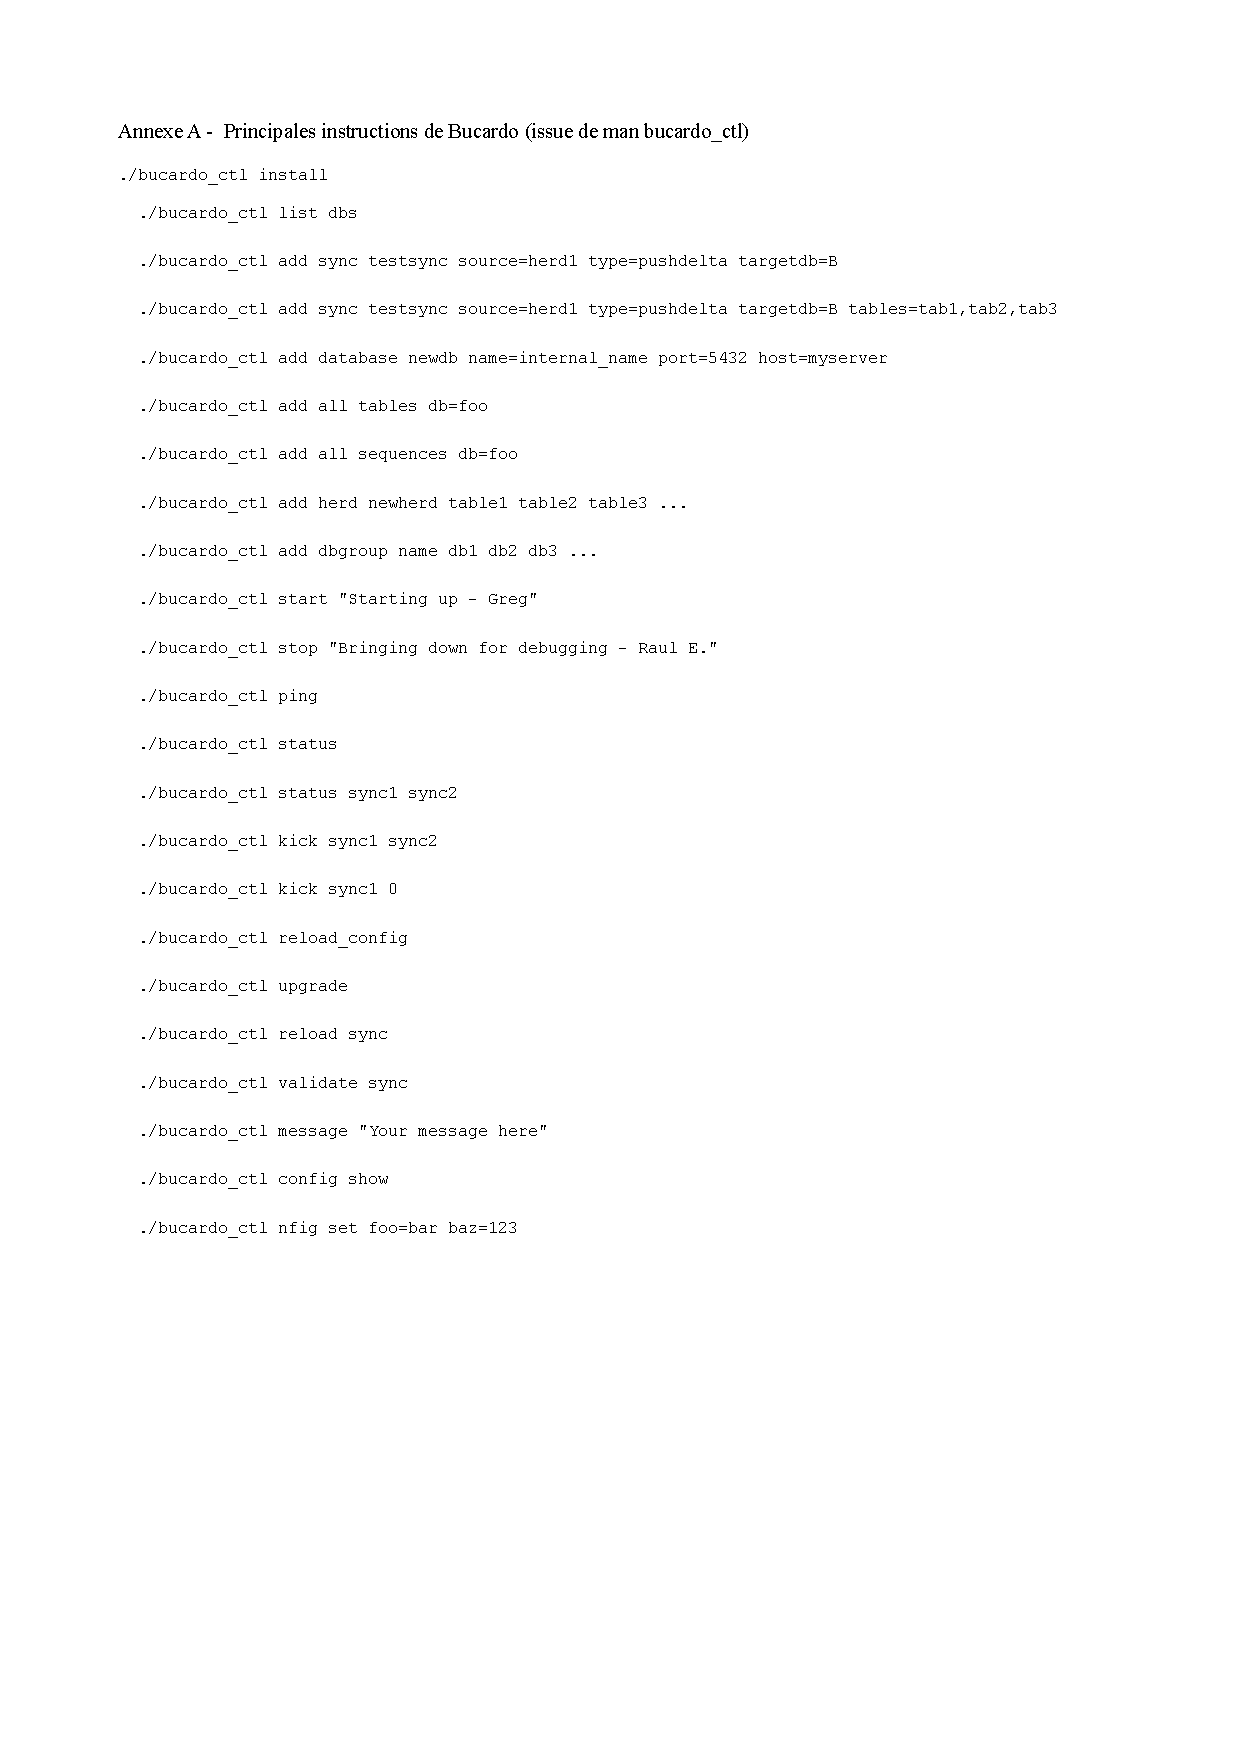
\includepdf[pages=1]{aa.pdf}

\section{Mise en œuvre détaillée de Bucardo}

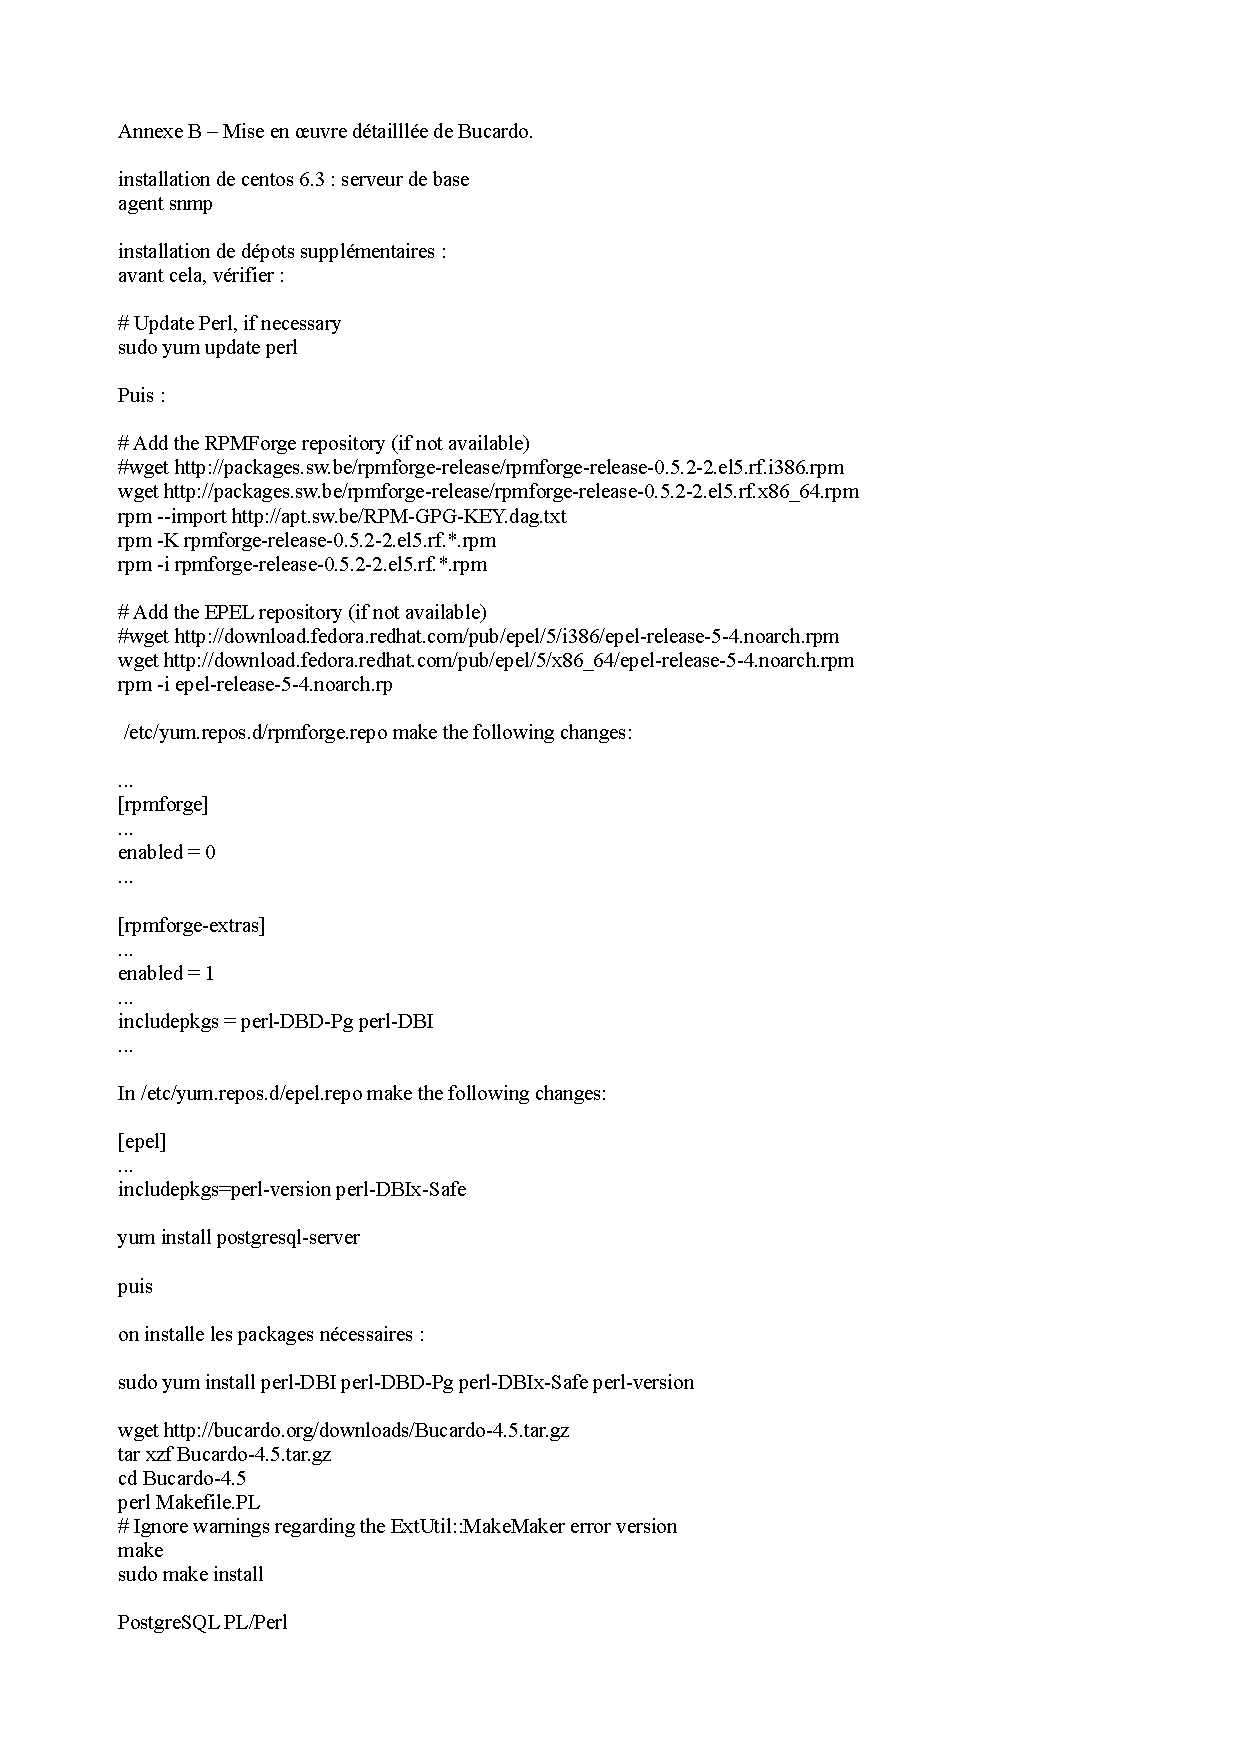
\includepdf[pages=1-17]{ab.pdf}

\section{Mise en œuvre de HAProxy et de pgBouncer}

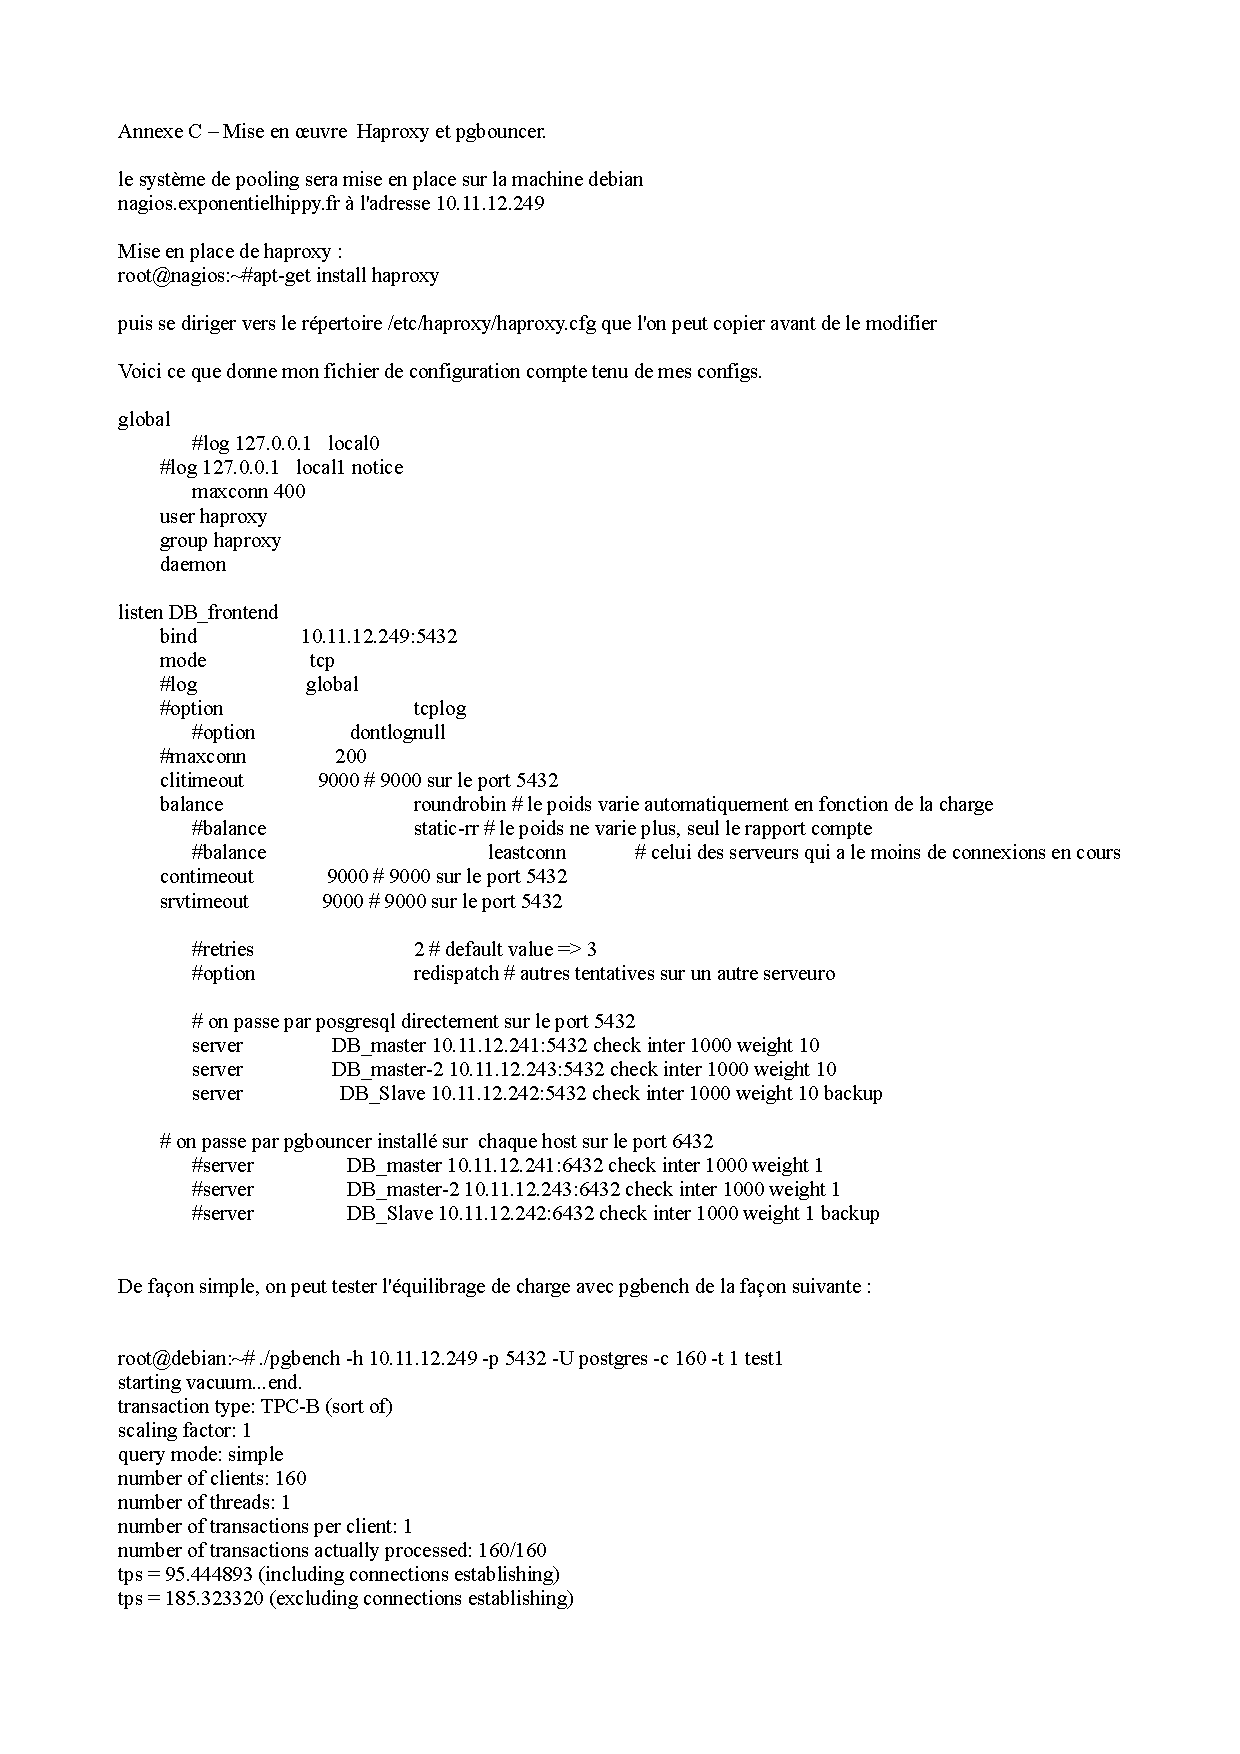
\includepdf[pages=1-6]{ac.pdf}

\section{Mise en œuvre de pgPool — script de déploiement}

Voir : \url{http://git.r.s.tremoureux.fr/postgresql-clustering/src}

\section{Tests de pgPool — performances et résistances à la charge}

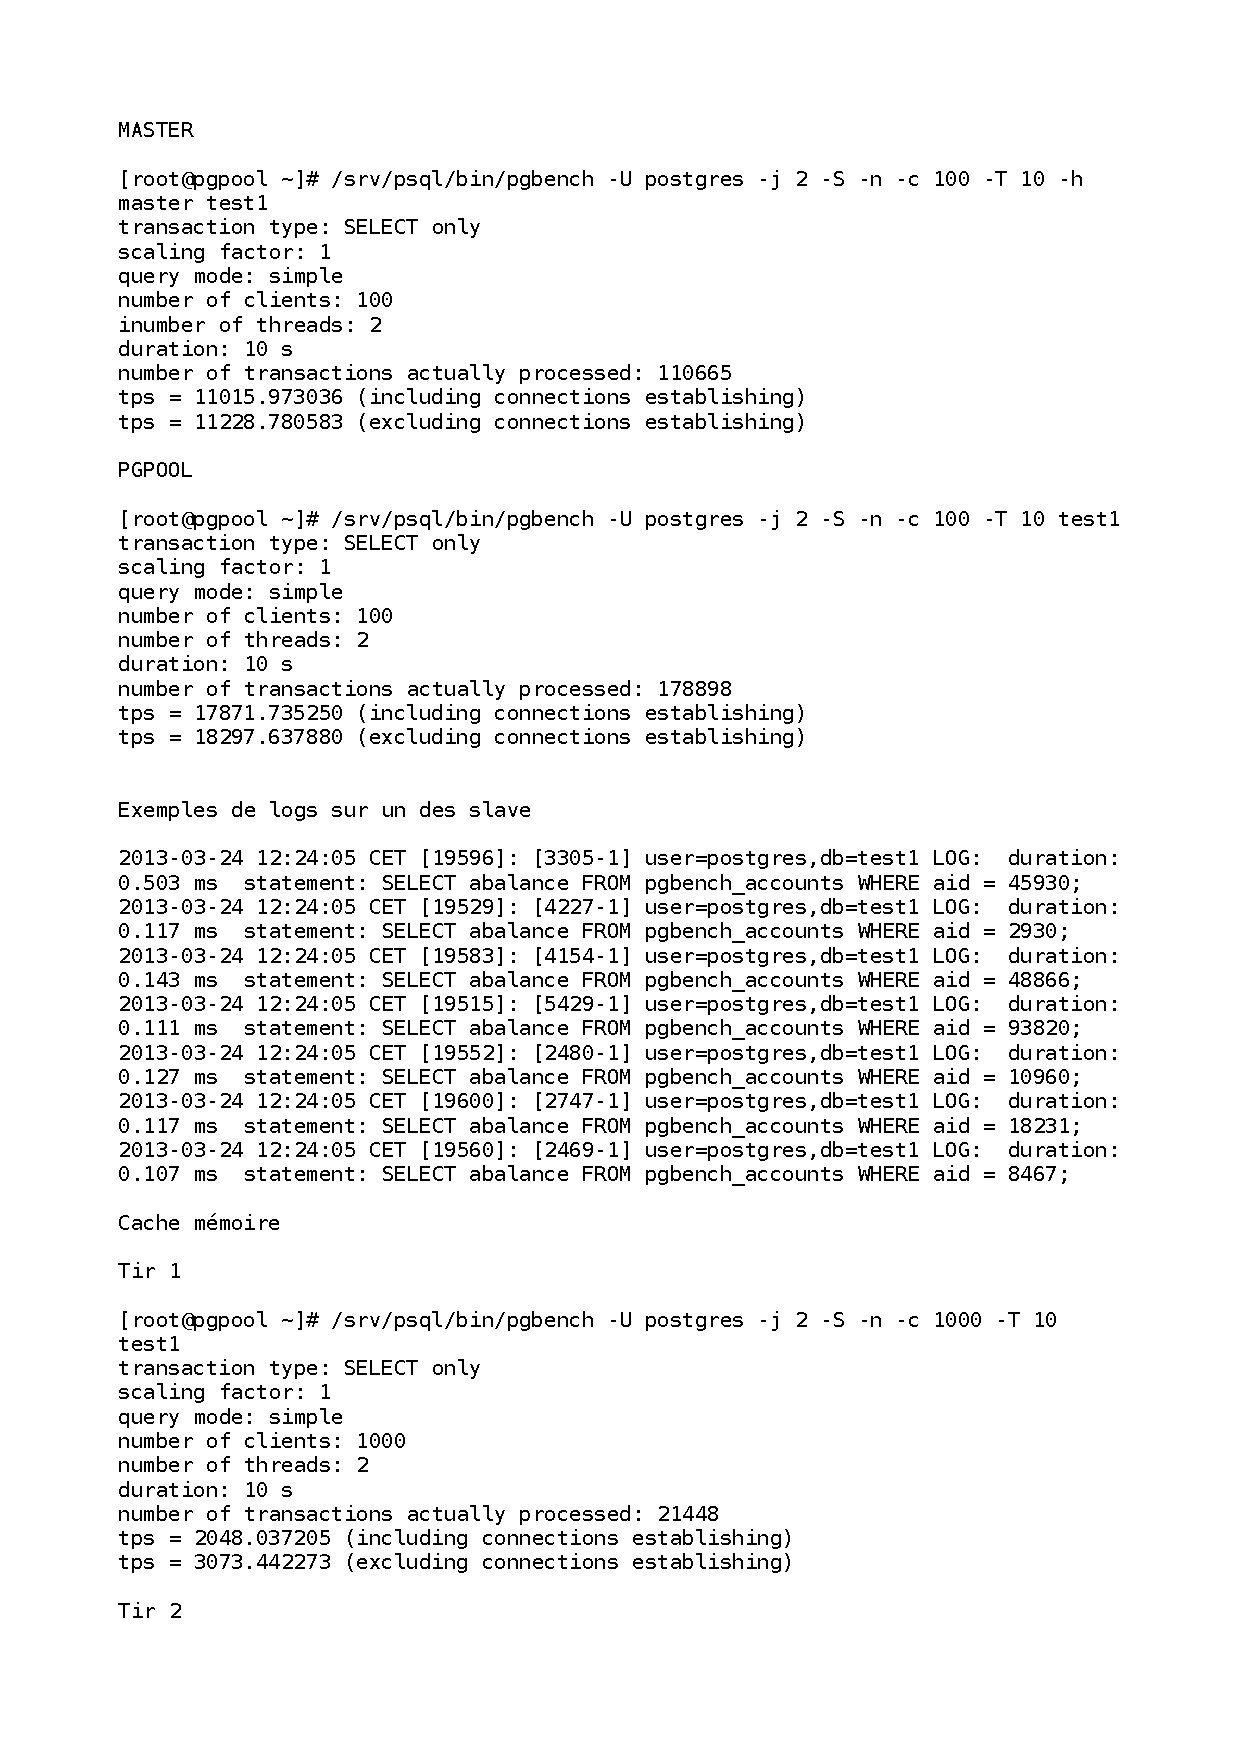
\includepdf[pages=1-5]{ae.pdf}


\end{document}
